\title{Taysols\\ ML model \\ train and deploy model Batch}
\author{Yiran Jing 
}
\date{June, 2019}
\documentclass[12pt]{article}
\usepackage[toc,page]{appendix}
\usepackage{graphicx} 
\usepackage{float}
\usepackage{caption}
\usepackage{subcaption}
\usepackage{geometry}
\usepackage{amsmath}
\usepackage{lscape}
\usepackage{natbib}
\usepackage{adjustbox}
\usepackage{changepage}
\usepackage{multicol}
\usepackage{booktabs}
\usepackage{hyperref}


\usepackage[dvipsnames]{xcolor}
\definecolor{mypink1}{rgb}{0.858, 0.188, 0.478}
\definecolor{mypink2}{cmyk}{0, 0.7808, 0.4429, 0.1412}
\definecolor{mygray}{gray}{0.6}
\colorlet{myorange}{green!10!orange!90!}

\geometry{
	a4paper,
	total={170mm,257mm},
	left=25mm,
	right=25mm,
	top=25mm,
	bottom=20mm}

\newcommand{\HRule}[1]{\rule{\linewidth}{#1}}
\setcounter{tocdepth}{5}
\setcounter{secnumdepth}{5}

\begin{document}

\title{ \normalsize \textsc{Taysols Data Science}
		\\ [2.0cm]
		\HRule{0.5pt} \\
		\LARGE \textbf{\uppercase{Building AWS Lambda Function on Machine Learning model}}
		\HRule{2pt} \\ [0.5cm]
		\small \textbf{Example of invoking Lambda Function on S3 PUT Event with Existing XGBoost Endpoint}
		\normalsize \vspace*{5\baselineskip}}
		
\date{July 05, 2019}
\author{Yiran Jing\\}
\maketitle

\pagenumbering{gobble}
\newpage
\thispagestyle{empty}

\newpage
\tableofcontents
\newpage
\setcounter{page}{1}
\pagenumbering{arabic}




\section{Introduction to Lambda Function}

Lambda Builders is a separate project that contains scripts to build Lambda functions, given a source location. Build Actions could be implemented in any programming language. Preferably in the language that they are building, I use Python as the DEMO example in this note. Also, the method in this notebook can be used both for hosting service and batch transformation.
\\
\\
\noindent
Basically \textbf{AWS Lambda} lets you focus on writing code and not dealing with annoying things like VPCs, EC2 instances, MySQL databases, etc. Just write some Python, give that code to Lambda, and it will execute that code in the Cloud. Even better, \textbf{you can trigger that code in a variety of ways}: every minute, once a day, when you put something into an S3 bucket, etc. In this case, I give an example of execute Lambda Function on S3 event trigger, that is, we can \textit{execute lambda function automatically on our built ML models when we push new dataset to S3 bucket}.
\\
\\
\noindent
After you write up your Lmabda Function, everyone can easily use it to run model on new dataset, and the user does not need to touch Sagemaker of Lambda function again. See figure \ref{fig:create_lambda_1} below:
\begin{figure}[H]
\centering
\begin{minipage}{1\textwidth}
  \centering
  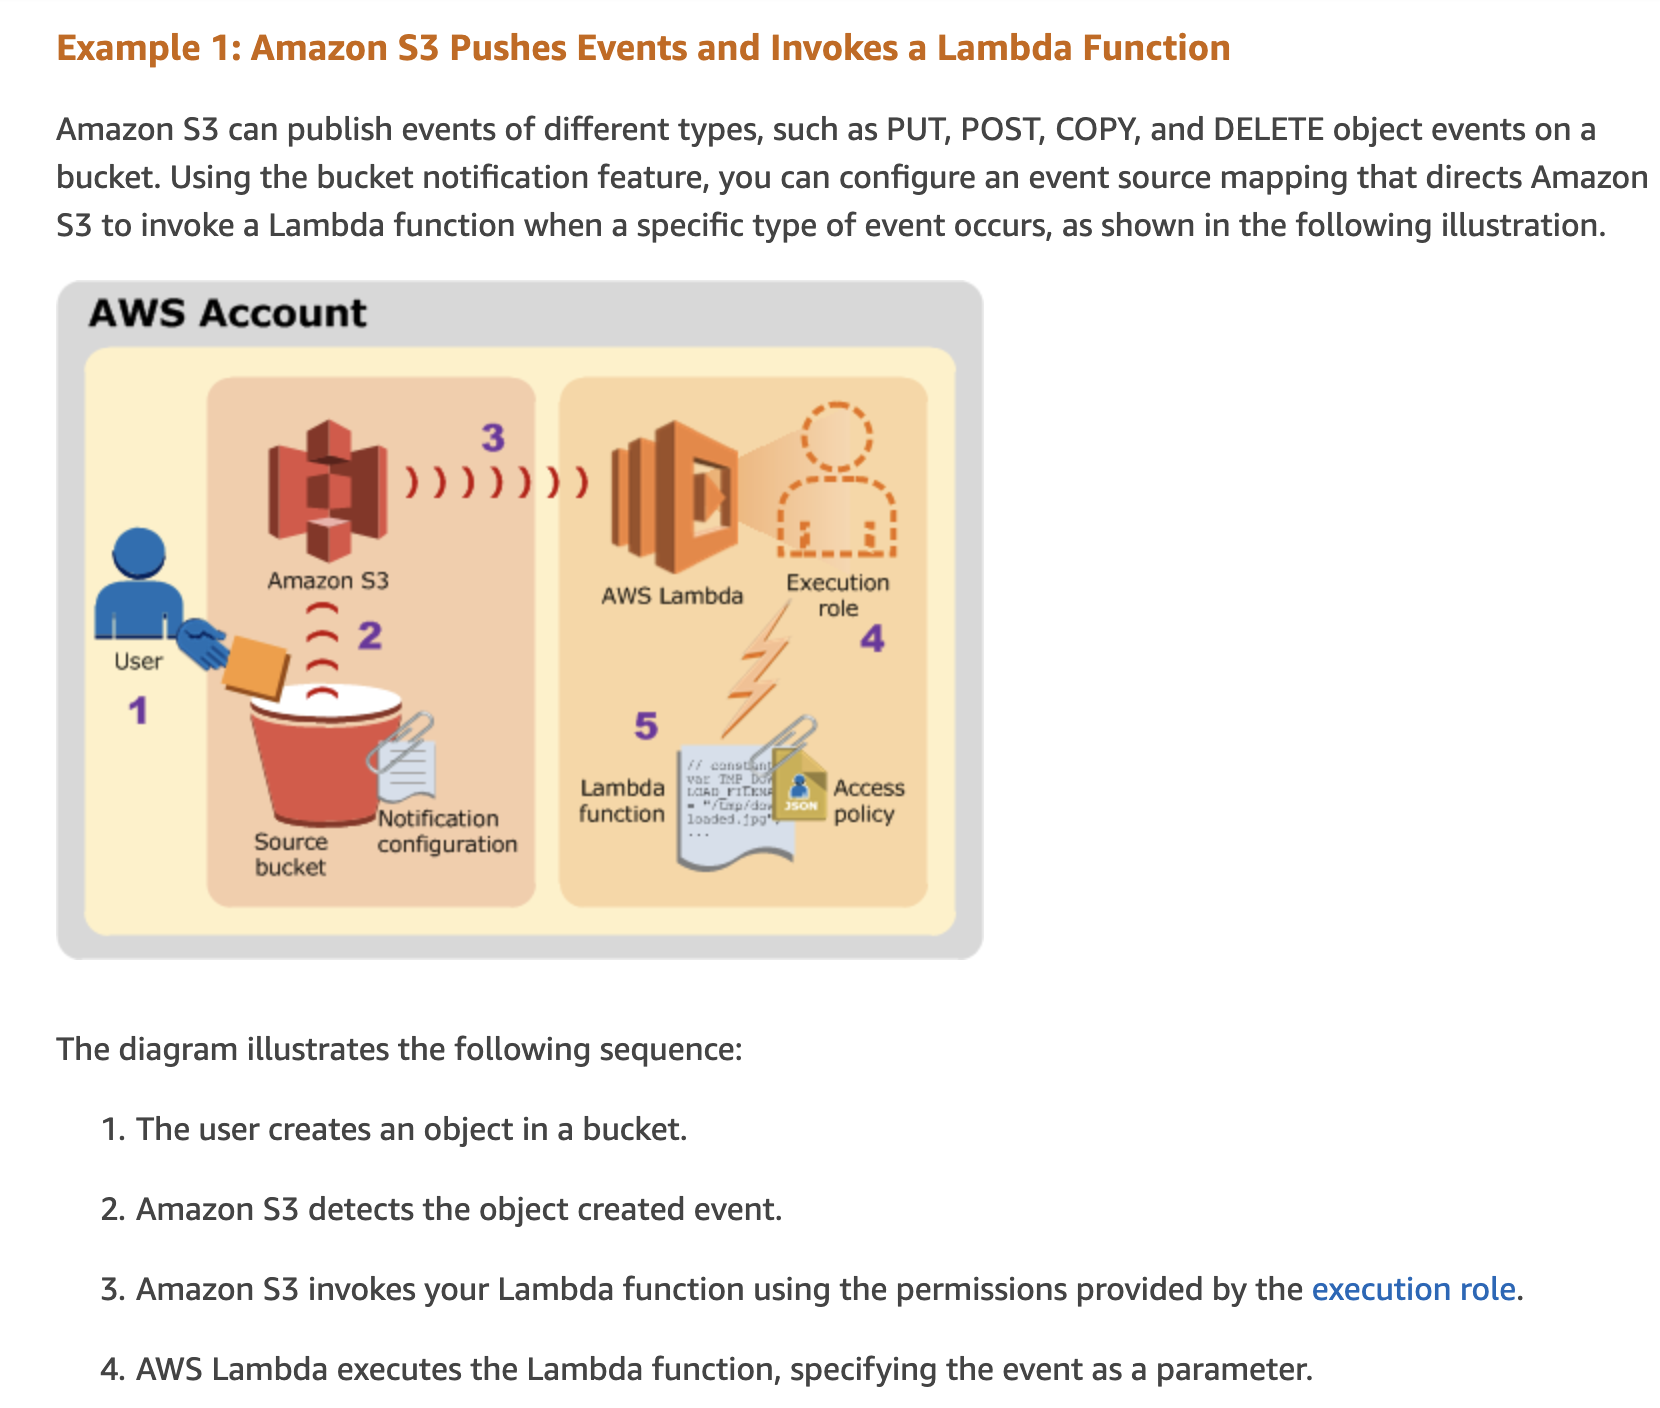
\includegraphics[width=1\linewidth]{TriggerS3Example.png}
   \caption{Example: Amazon S3 Pushes Events and Invokes a Lambda Function}
   \label{fig:TriggerS3Example}
\end{minipage}%
\end{figure}
\noindent



\newpage
\section{Clean data within Lambda Function}
\subsection{Install AWS Lambda with Pandas and NumPy}
AWS Lambda does not include Pandas/NumPy Python libraries by default. But we do need use Pandas and NumPy with Lambda functions for data cleaning and transformation. \href{https://medium.com/@korniichuk/lambda-with-pandas-fd81aa2ff25e}{\textit{click me to see how to do it}}

\subsection{Write python script to manipulate raw data}
%%%%%%% havenot done !

\subsection{Combine python script to Lambda Function}
%%%%%%% havenot done !



\newpage
\section{Create an IAM role that grants access to the S3 bucket}

Before you get started building your Lambda function, you must first create an IAM role which Lambda will use to work with S3 and to write logs to CloudWatch. This role should be set up with the appropriate S3 and CloudWatch policies.See figure \ref{fig:create_role}, select Lambda and click \textit{Next: Permission}.
\begin{figure}[H]
\centering
\begin{minipage}{1\textwidth}
  \centering
  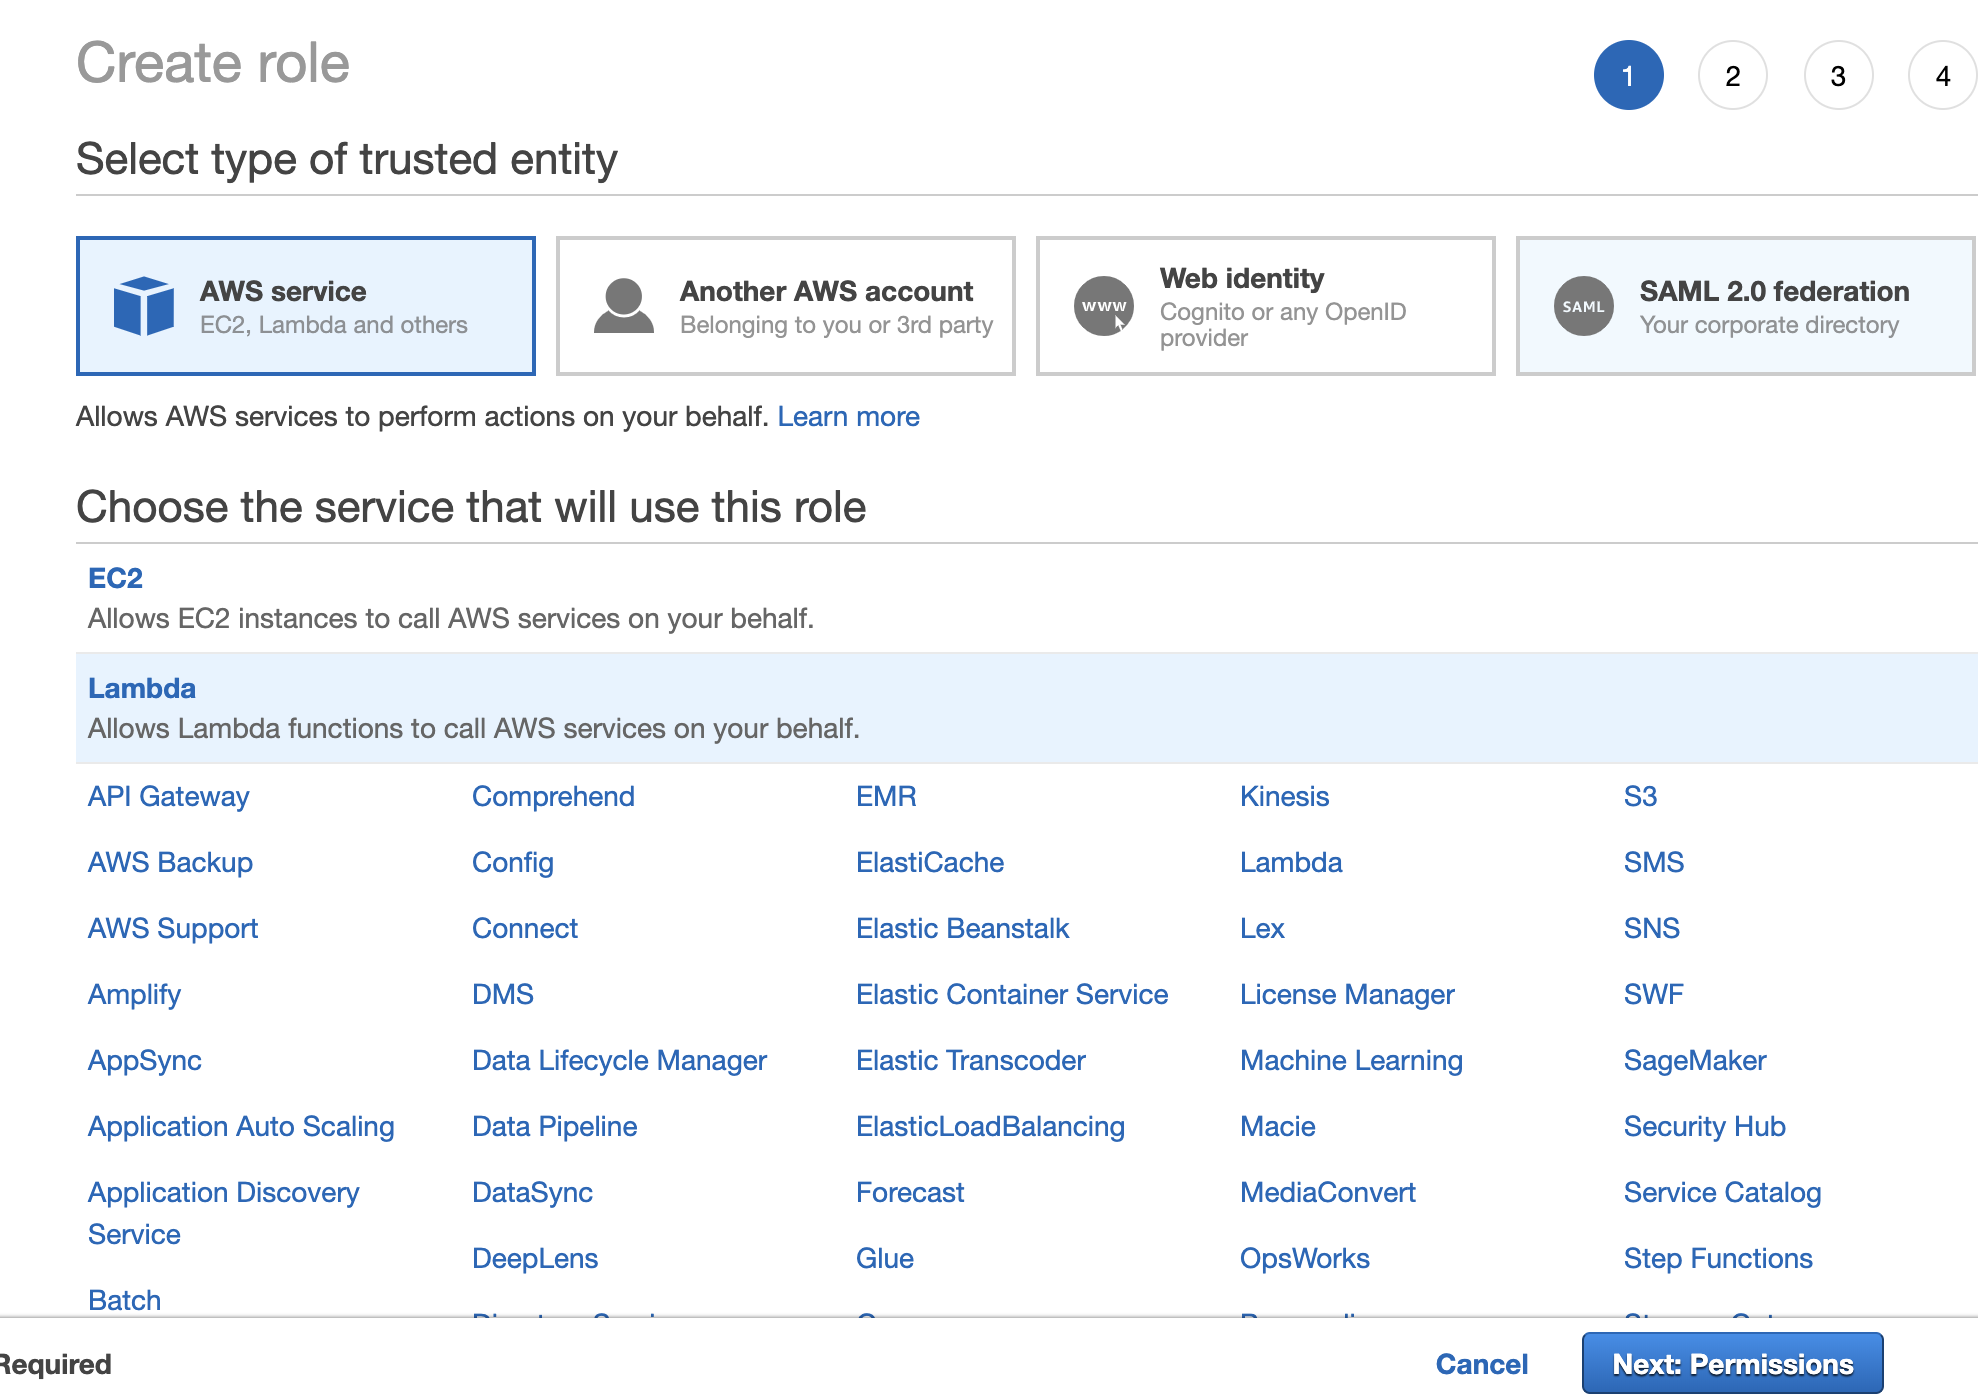
\includegraphics[width=1\linewidth]{create_role.png}
   \caption{Create role steps}
   \label{fig:create_role}
\end{minipage}%
\end{figure}

\noindent
And then you need to select three pollicies\textit{\textbf{AWSLambdaFullAccess, AmazonS3FullAccess and AmazonSageMakerFullAccess}}, also you need give \textbf{CloudWatchPermission} by \textbf{adding inline policy with Json Format} after you create the role: 
See figure \ref{fig:Role_example} and figure \ref{fig:role_example_2}. \href{https://console.aws.amazon.com/iam/home?region=ap-southeast-2#/roles/Lambda_Permission_endpoint}{\textit{Click me to look the details of }\textbf{\textit{Lambda\_Permission\_endpoint}}}.

\begin{figure}[H]
\centering
\begin{minipage}{1\textwidth}
  \centering
  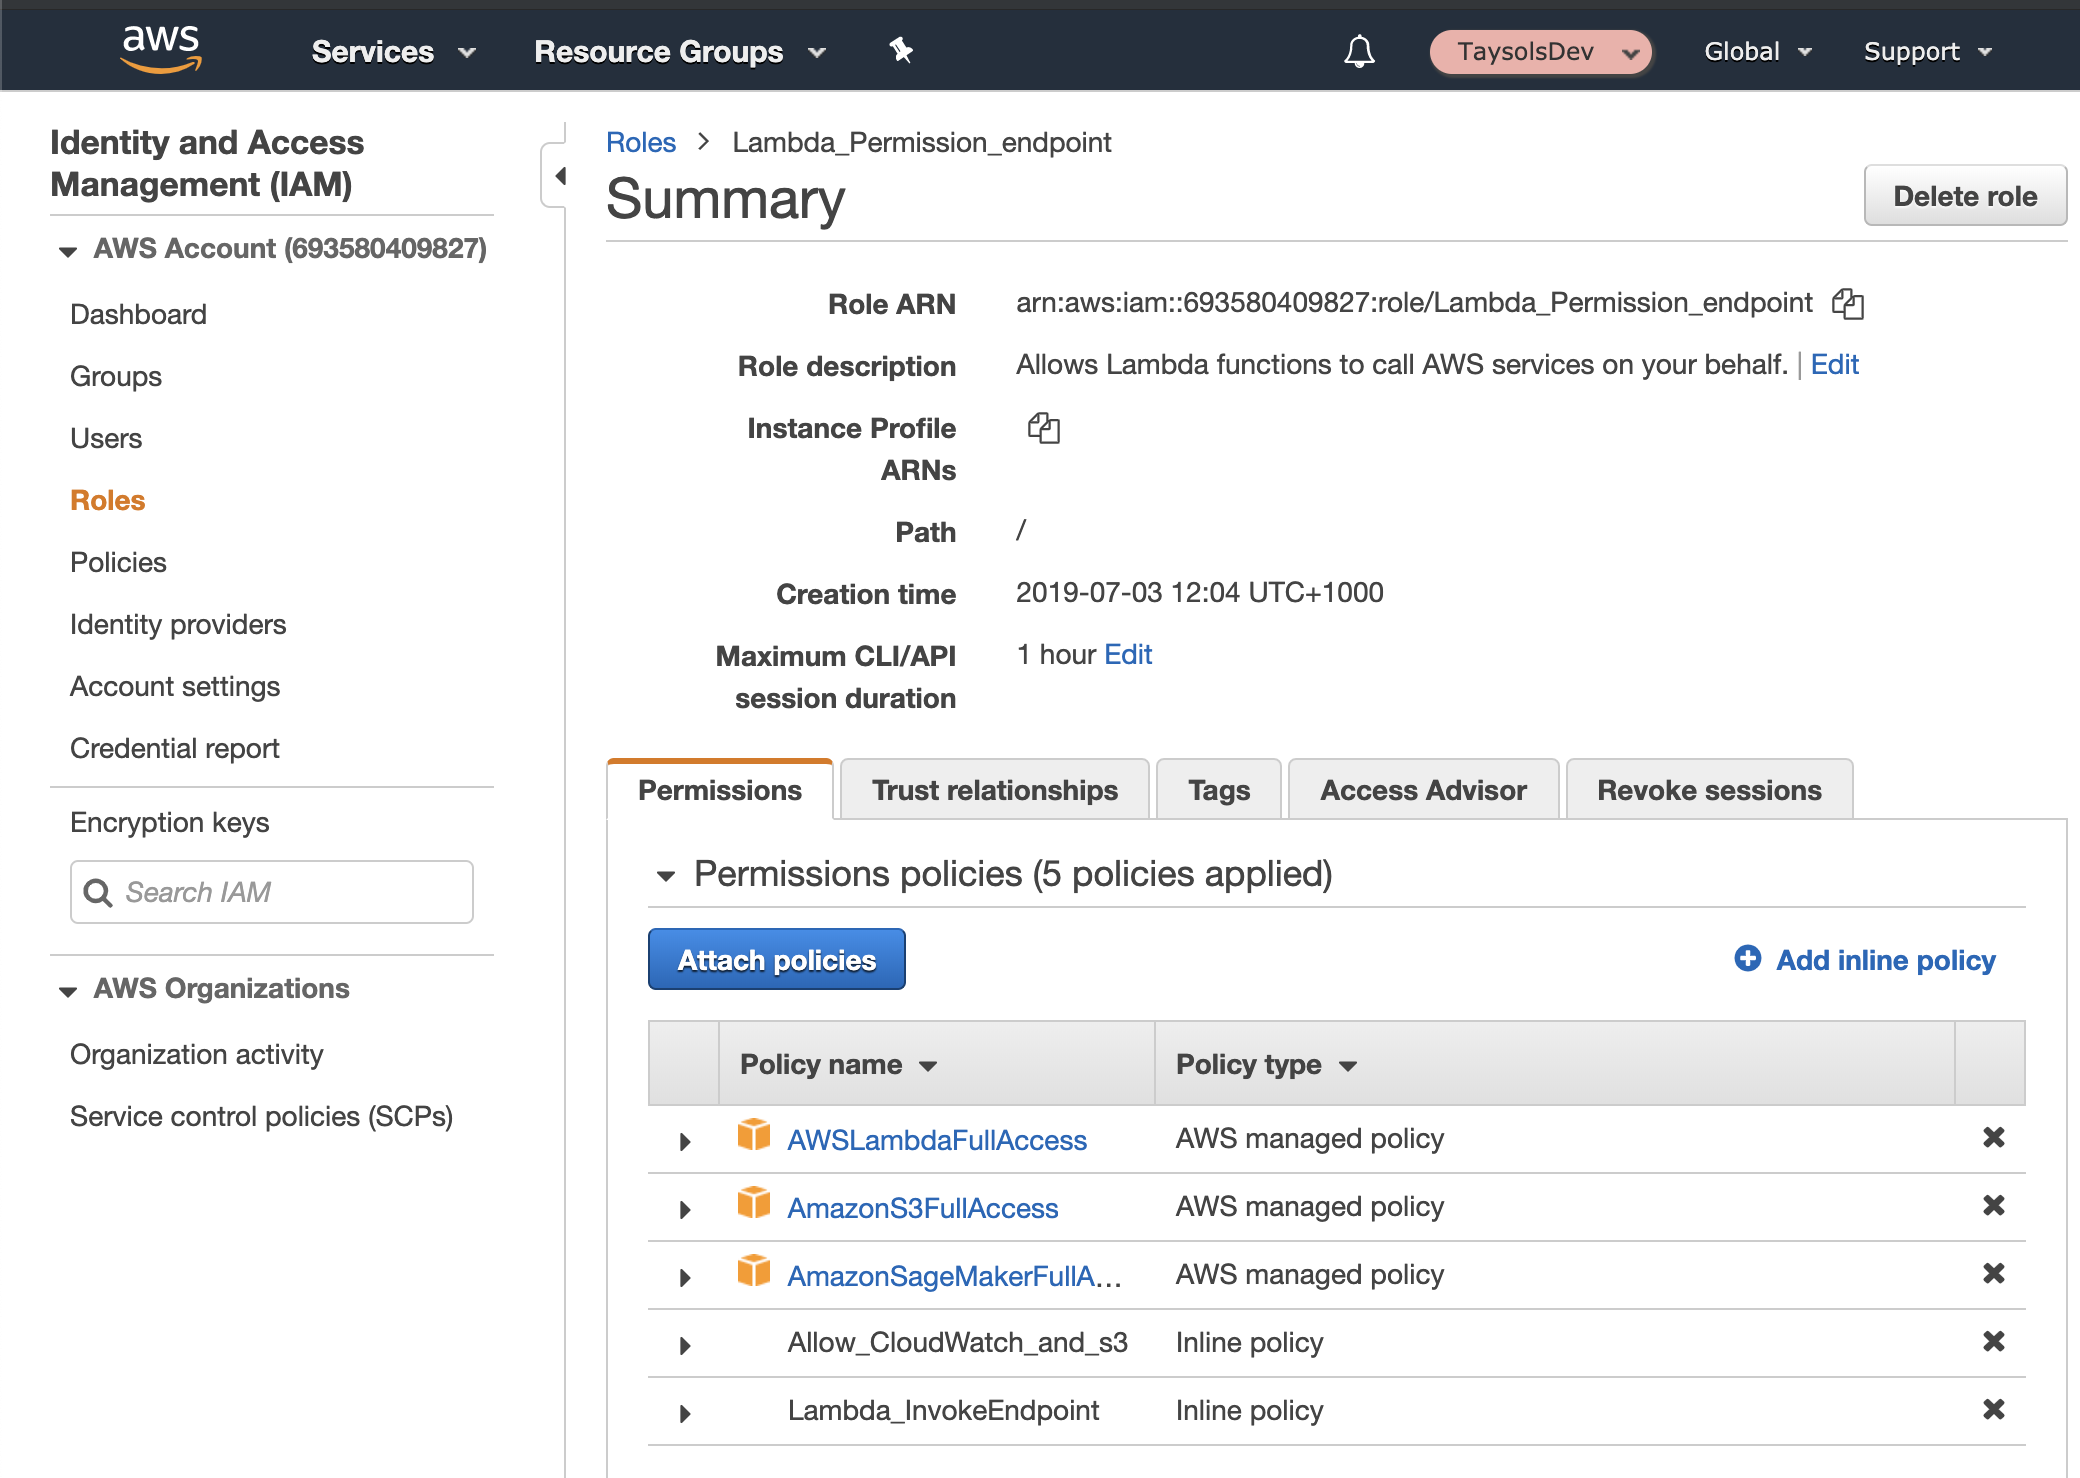
\includegraphics[width=1\linewidth]{Role_example.png}
   \caption{IAM role's policy: AWSLambdaFullAccess, AmazonS3FullAccess and AmazonSageMakerFullAccess}
   \label{fig:Role_example}
\end{minipage}%
\end{figure}

\begin{figure}[H]
\centering
\begin{minipage}{0.6\textwidth}
  \centering
  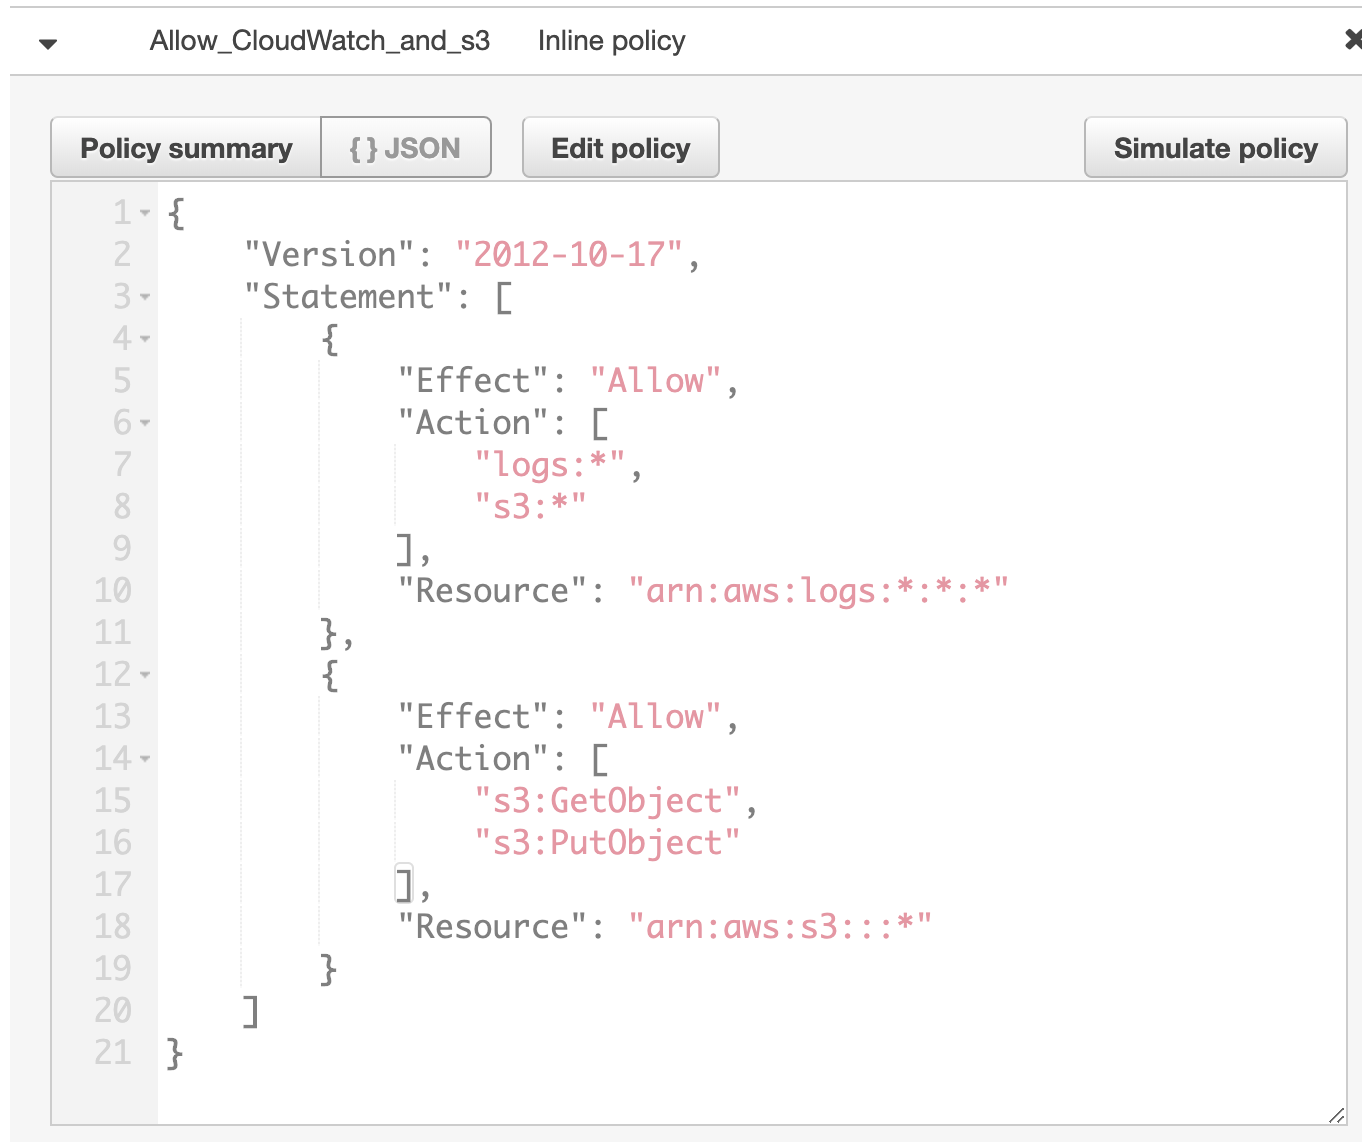
\includegraphics[width=1\linewidth]{role_example_2.png}
   \caption{IAM role's policy: CloudWatchPermission}
   \label{fig:role_example_2}
\end{minipage}%
\end{figure}




\newpage
\section{Create an empty Lambda function}
After we have a SageMaker model endpoint, for further usage of modelling we need to do is to Create a Lambda function that calls the SageMaker Runtime Invoke\_Endpoint
\noindent
See figure \ref{fig:create_lambda_1}, click \textit{create function}

\begin{figure}[H]
\centering
\begin{minipage}{1\textwidth}
  \centering
  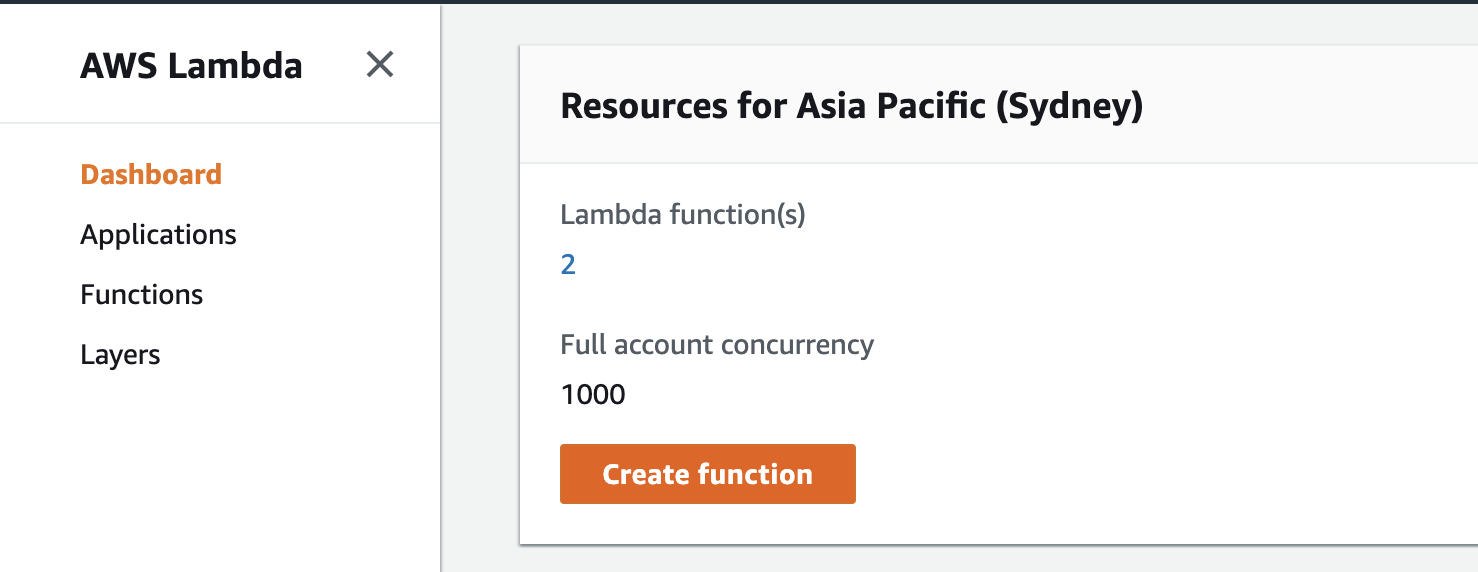
\includegraphics[width=1\linewidth]{create_lambda_1.png}
   \caption{Create a new Lambda Function from Amazon User Interface}
   \label{fig:create_lambda_1}
\end{minipage}%
\end{figure}
\noindent

\noindent
After that, give the name and language for your lambda funcation, see figure \ref{fig:create_lambda_2}. Please select \textbf{Python 3.6} and \textbf{Use an existing role}, then select the role which you created before. In this example, the IAM role I created in the last step is \textit{Lambda\_Permission\_endpoint}.
\begin{figure}[H]
\centering
\begin{minipage}{1\textwidth}
  \centering
  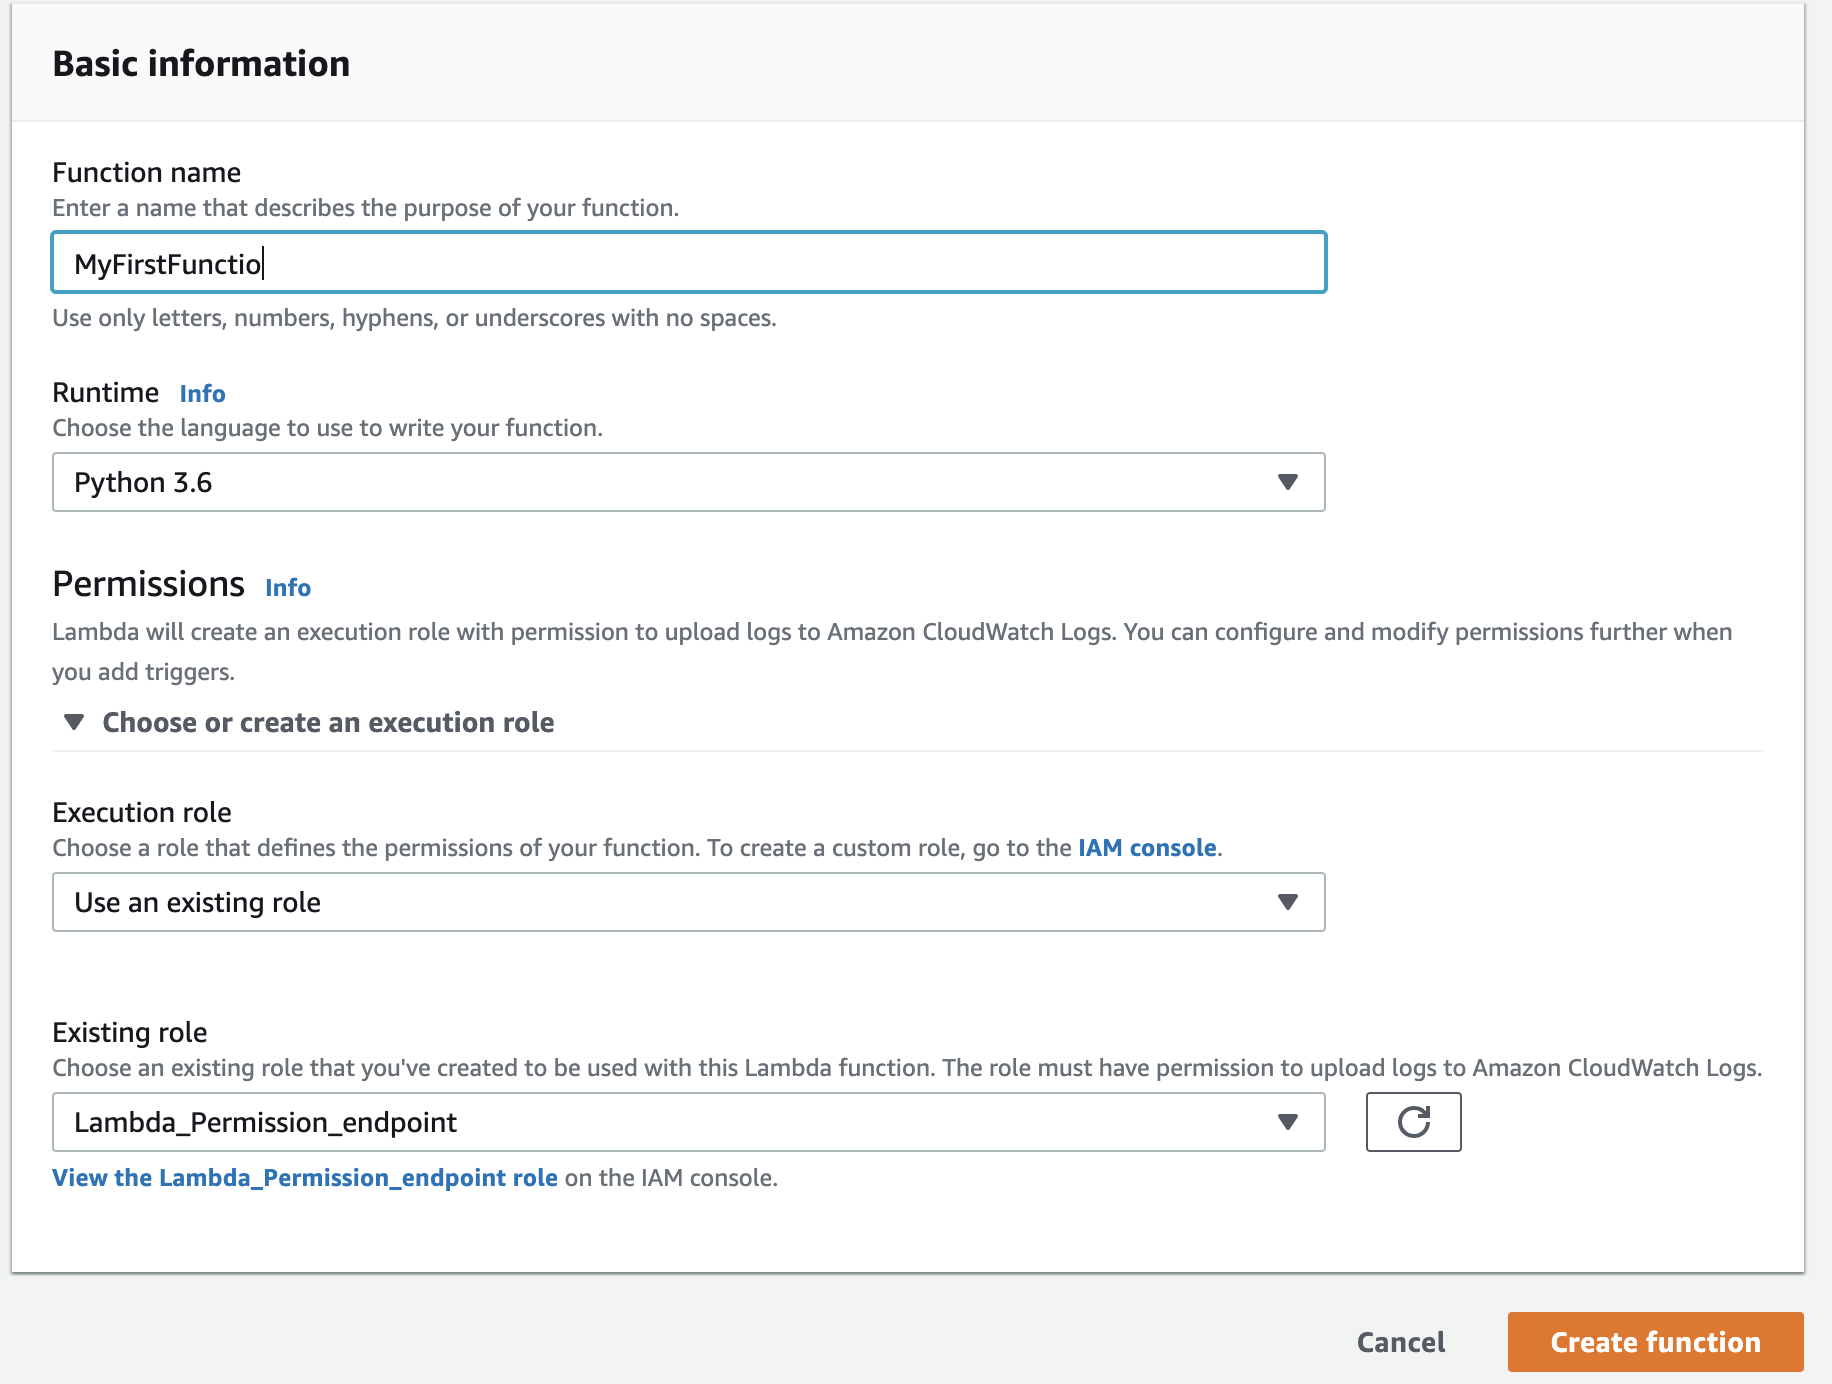
\includegraphics[width=1\linewidth]{create_lambda_2.png}
   \caption{Give the name and choice the language for your lambda function}
   \label{fig:create_lambda_2}
\end{minipage}%
\end{figure}

\noindent
Then, you can check the lambda function you have create a new lambda function through AWS Lambda interface, see figure \ref{fig:check_function}. 

\begin{figure}[H]
\centering
\begin{minipage}{1\textwidth}
  \centering
  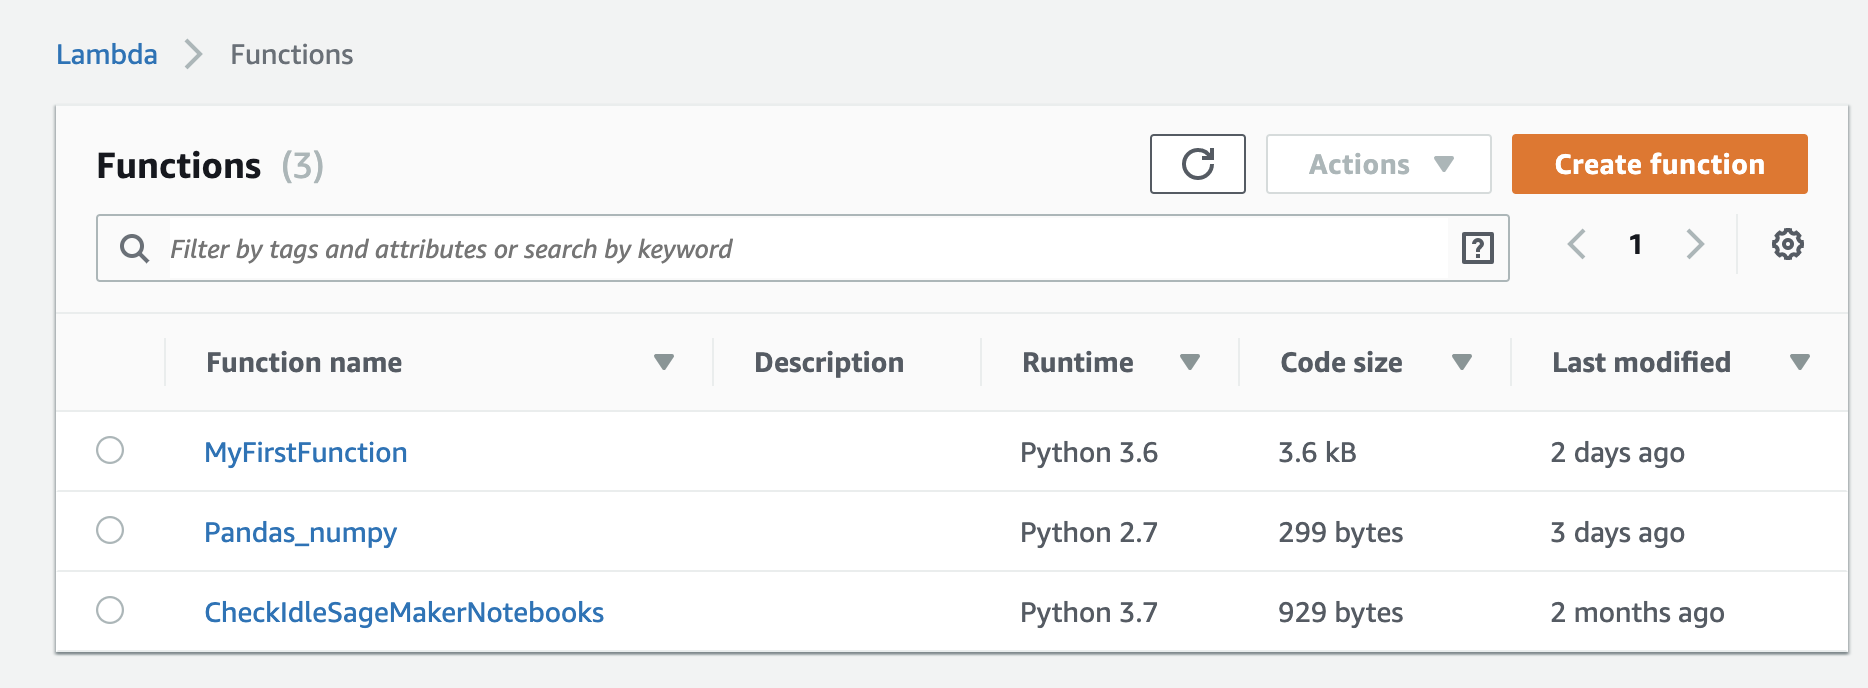
\includegraphics[width=1\linewidth]{check_function.png}
   \caption{Check you have create a new lambda function}
   \label{fig:check_function}
\end{minipage}%
\end{figure}


\newpage
\section{Build your Lambda Function}

For the following steps, Please remember that every time you \textbf{must click \textit{save} } before click \textit{test}  to running the new code on your \textit{test event}.

\subsection{S3 Event Triggers}
After you create a new empty Lambda function, the next step is add \textbf{S3 put} as event trigger. Click \textbf{add triggers}
See figure \ref{fig:build_lambda_1}. select S3 \textbf{PUT} as trigger event, then Enter prefix, in case if you have any folders inside the S3 and want to triggered only uploading to that folder. In our example, the \textbf{Prefix is the path of the file containing input dataset}. Suffix is \textbf{.csv} since our dataset is csv. 
\begin{figure}[H]
\centering
\begin{minipage}{1\textwidth}
  \centering
  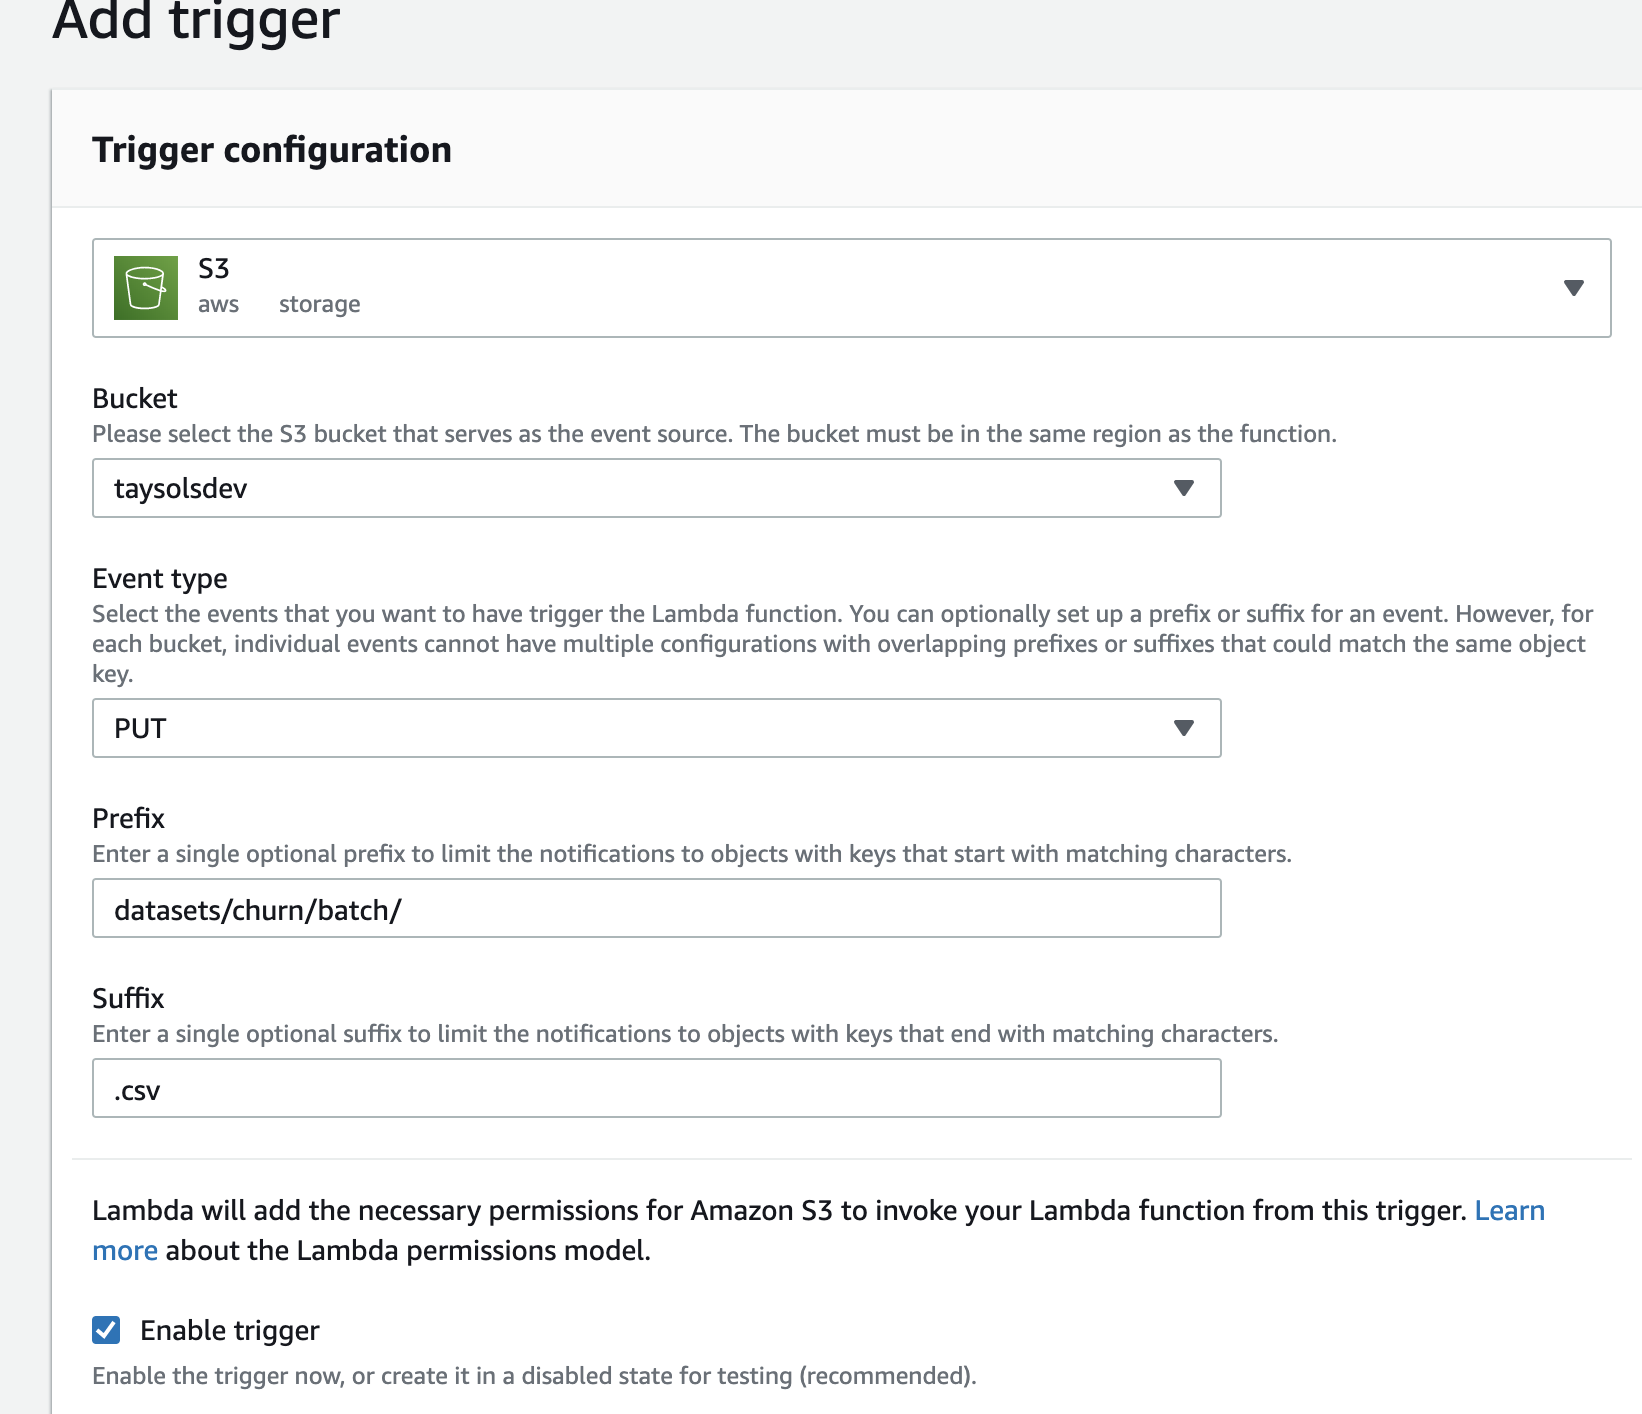
\includegraphics[width=1\linewidth]{build_lambda_1.png}
   \caption{Select S3 put as event trigger}
   \label{fig:build_lambda_1}
\end{minipage}%
\end{figure}
After that, check your lambda function, it should look like figure \ref{fig:build_lambda_2}.:

\begin{figure}[H]
\centering
\begin{minipage}{1\textwidth}
  \centering
  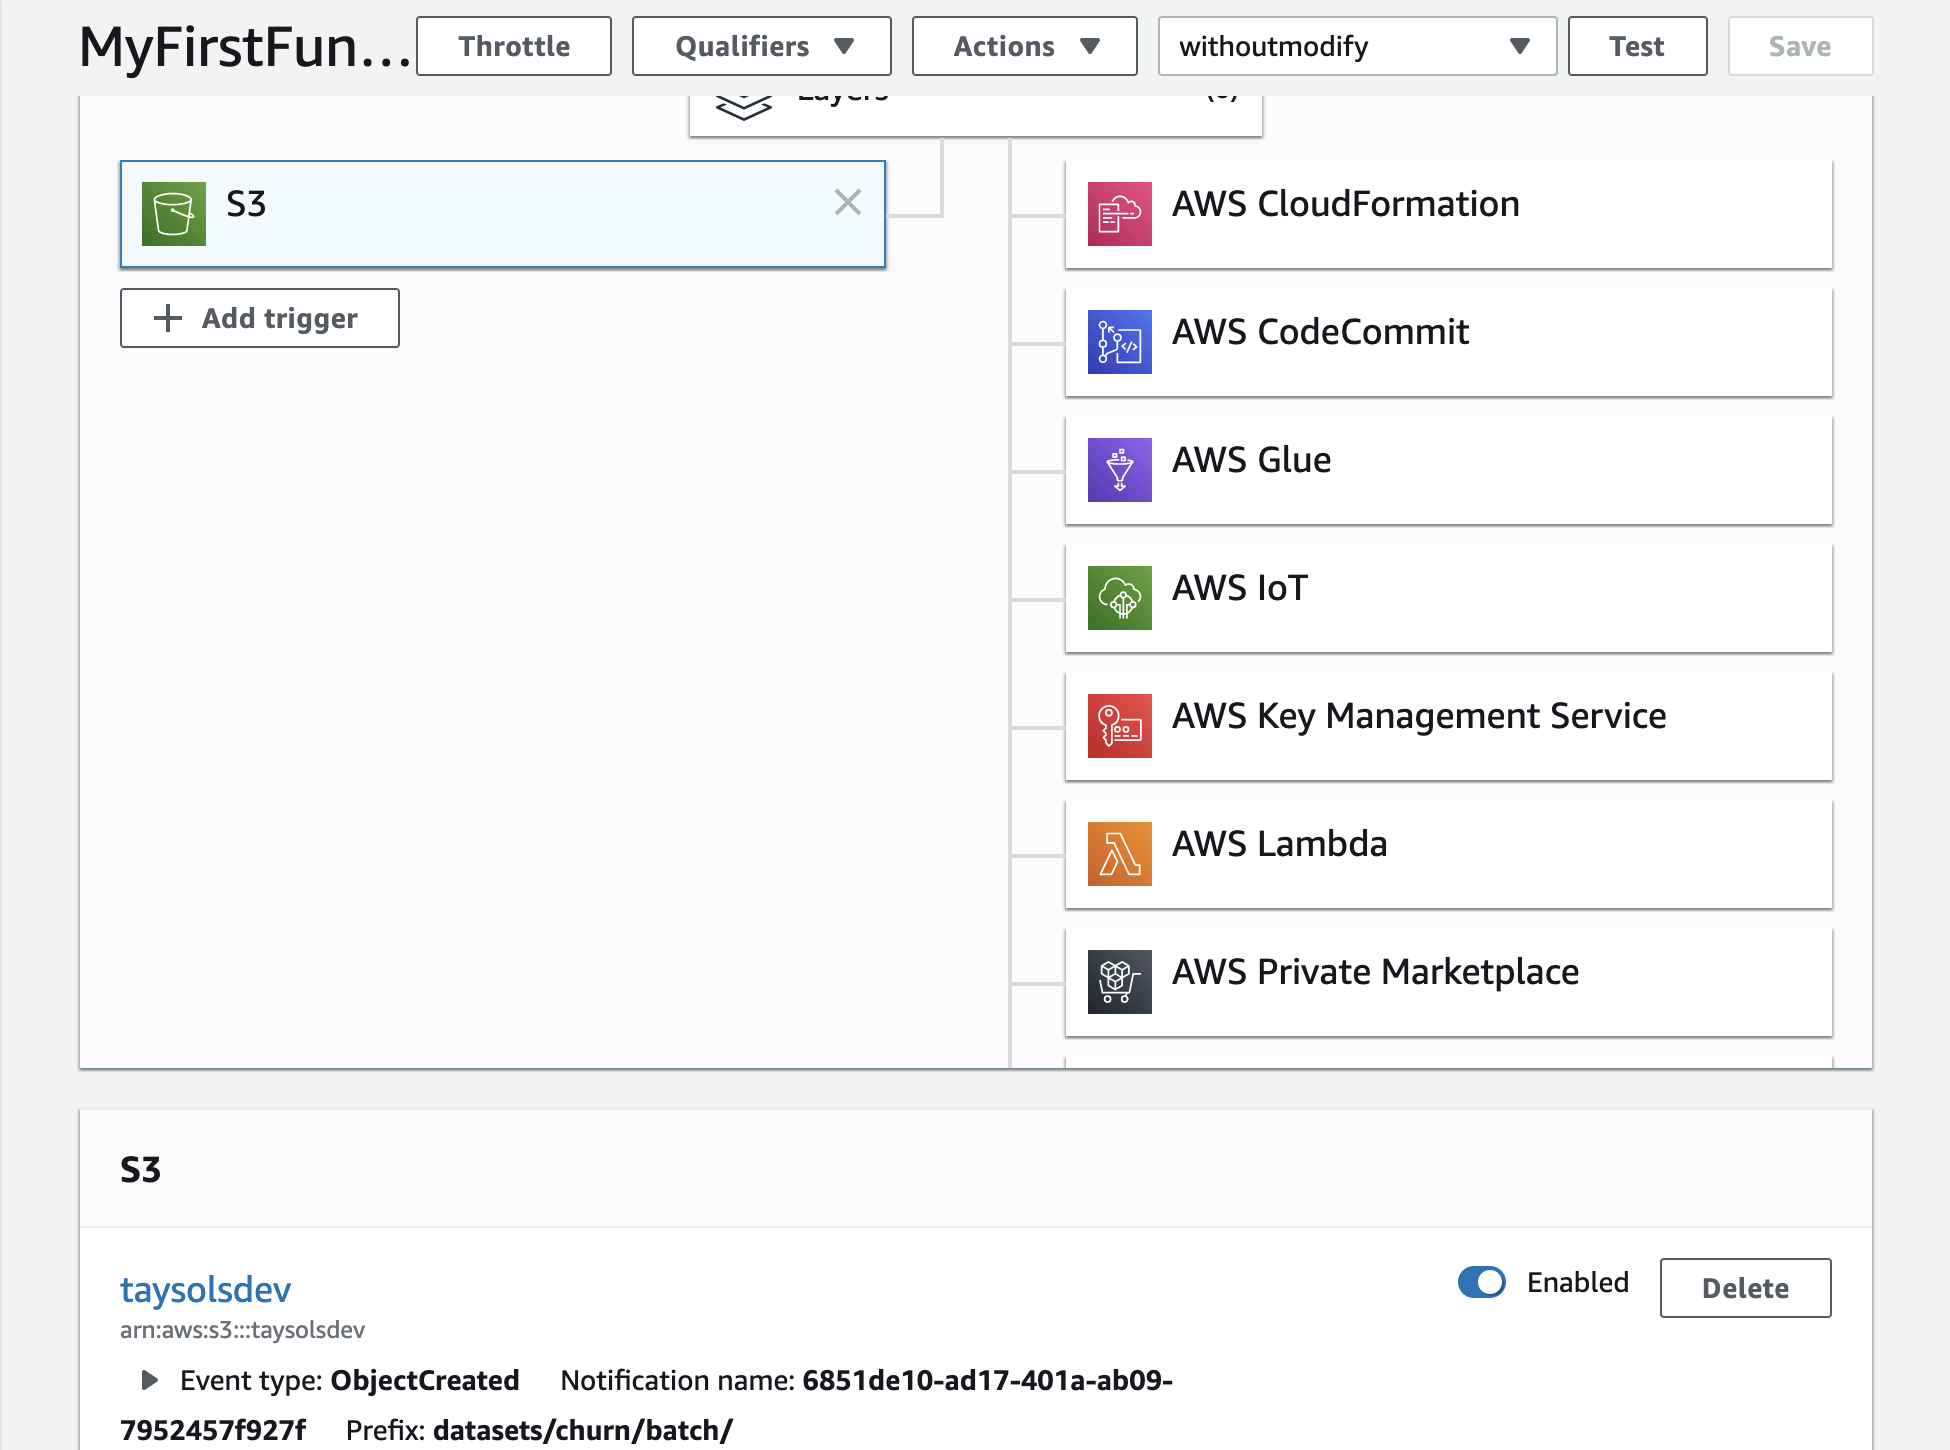
\includegraphics[width=1\linewidth]{build_lambda_2.png}
   \caption{your lambda function}
   \label{fig:build_lambda_2}
\end{minipage}%
\end{figure}


\subsection{Input environment variable}
\textbf{ENDPOINT\_NAME} is an environment variable that holds the name of the SageMaker model endpoint you just deployed using the sample notebook as shown in the following screenshot figure \ref{fig:envir_vari}:

\begin{figure}[H]
\centering
\begin{minipage}{1\textwidth}
  \centering
  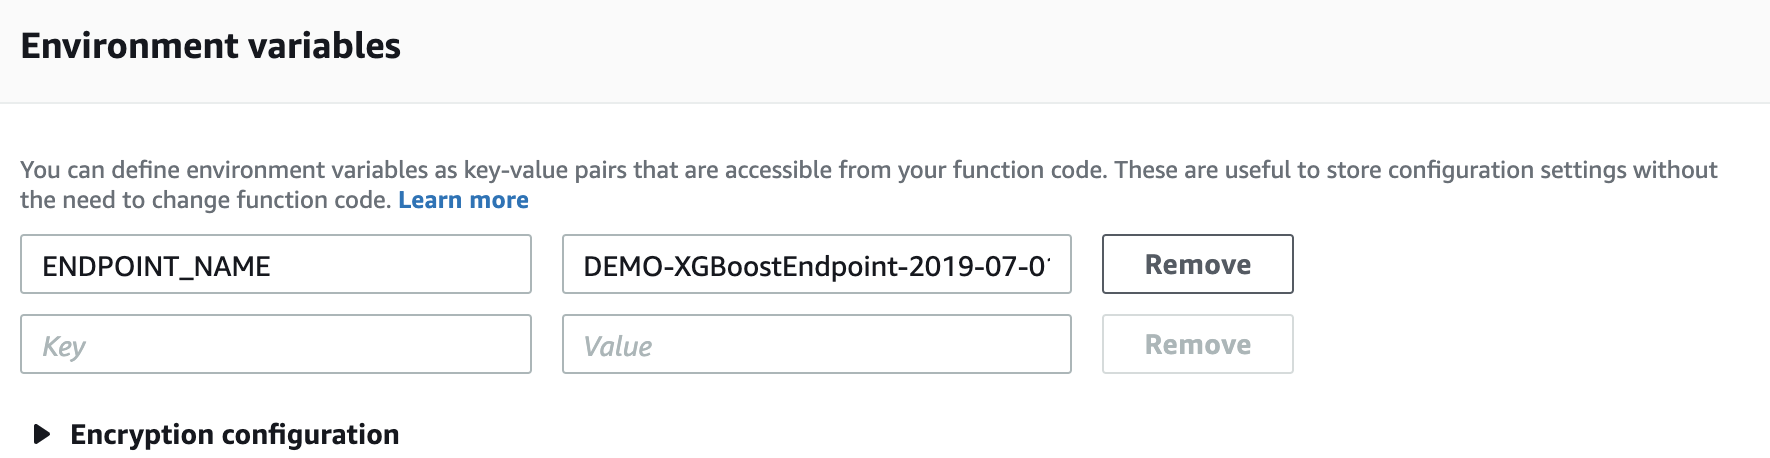
\includegraphics[width=1\linewidth]{envir_vari.png}
   \caption{Add endpoint of model to your Lambda Function}
   \label{fig:envir_vari}
\end{minipage}%
\end{figure}
\noindent
You can also modify or delete S3 event trigger in S3 bucket. See figure \ref{fig:S3_bucket_event_1} and figure \ref{fig:S3_bucket_event_2}:

\begin{figure}[H]
\centering
\begin{minipage}{1\textwidth}
  \centering
  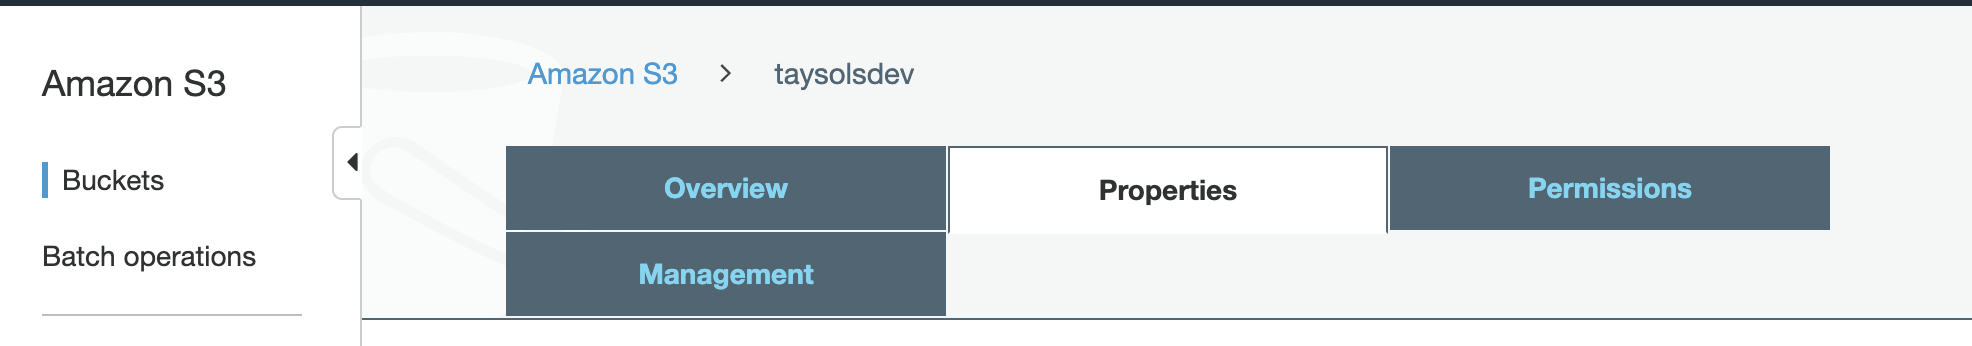
\includegraphics[width=1\linewidth]{S3_bucket_event_1.png}
   \caption{}
   \label{fig:S3_bucket_event_1}
\end{minipage}%
\end{figure}

\begin{figure}[H]
\centering
\begin{minipage}{1\textwidth}
  \centering
  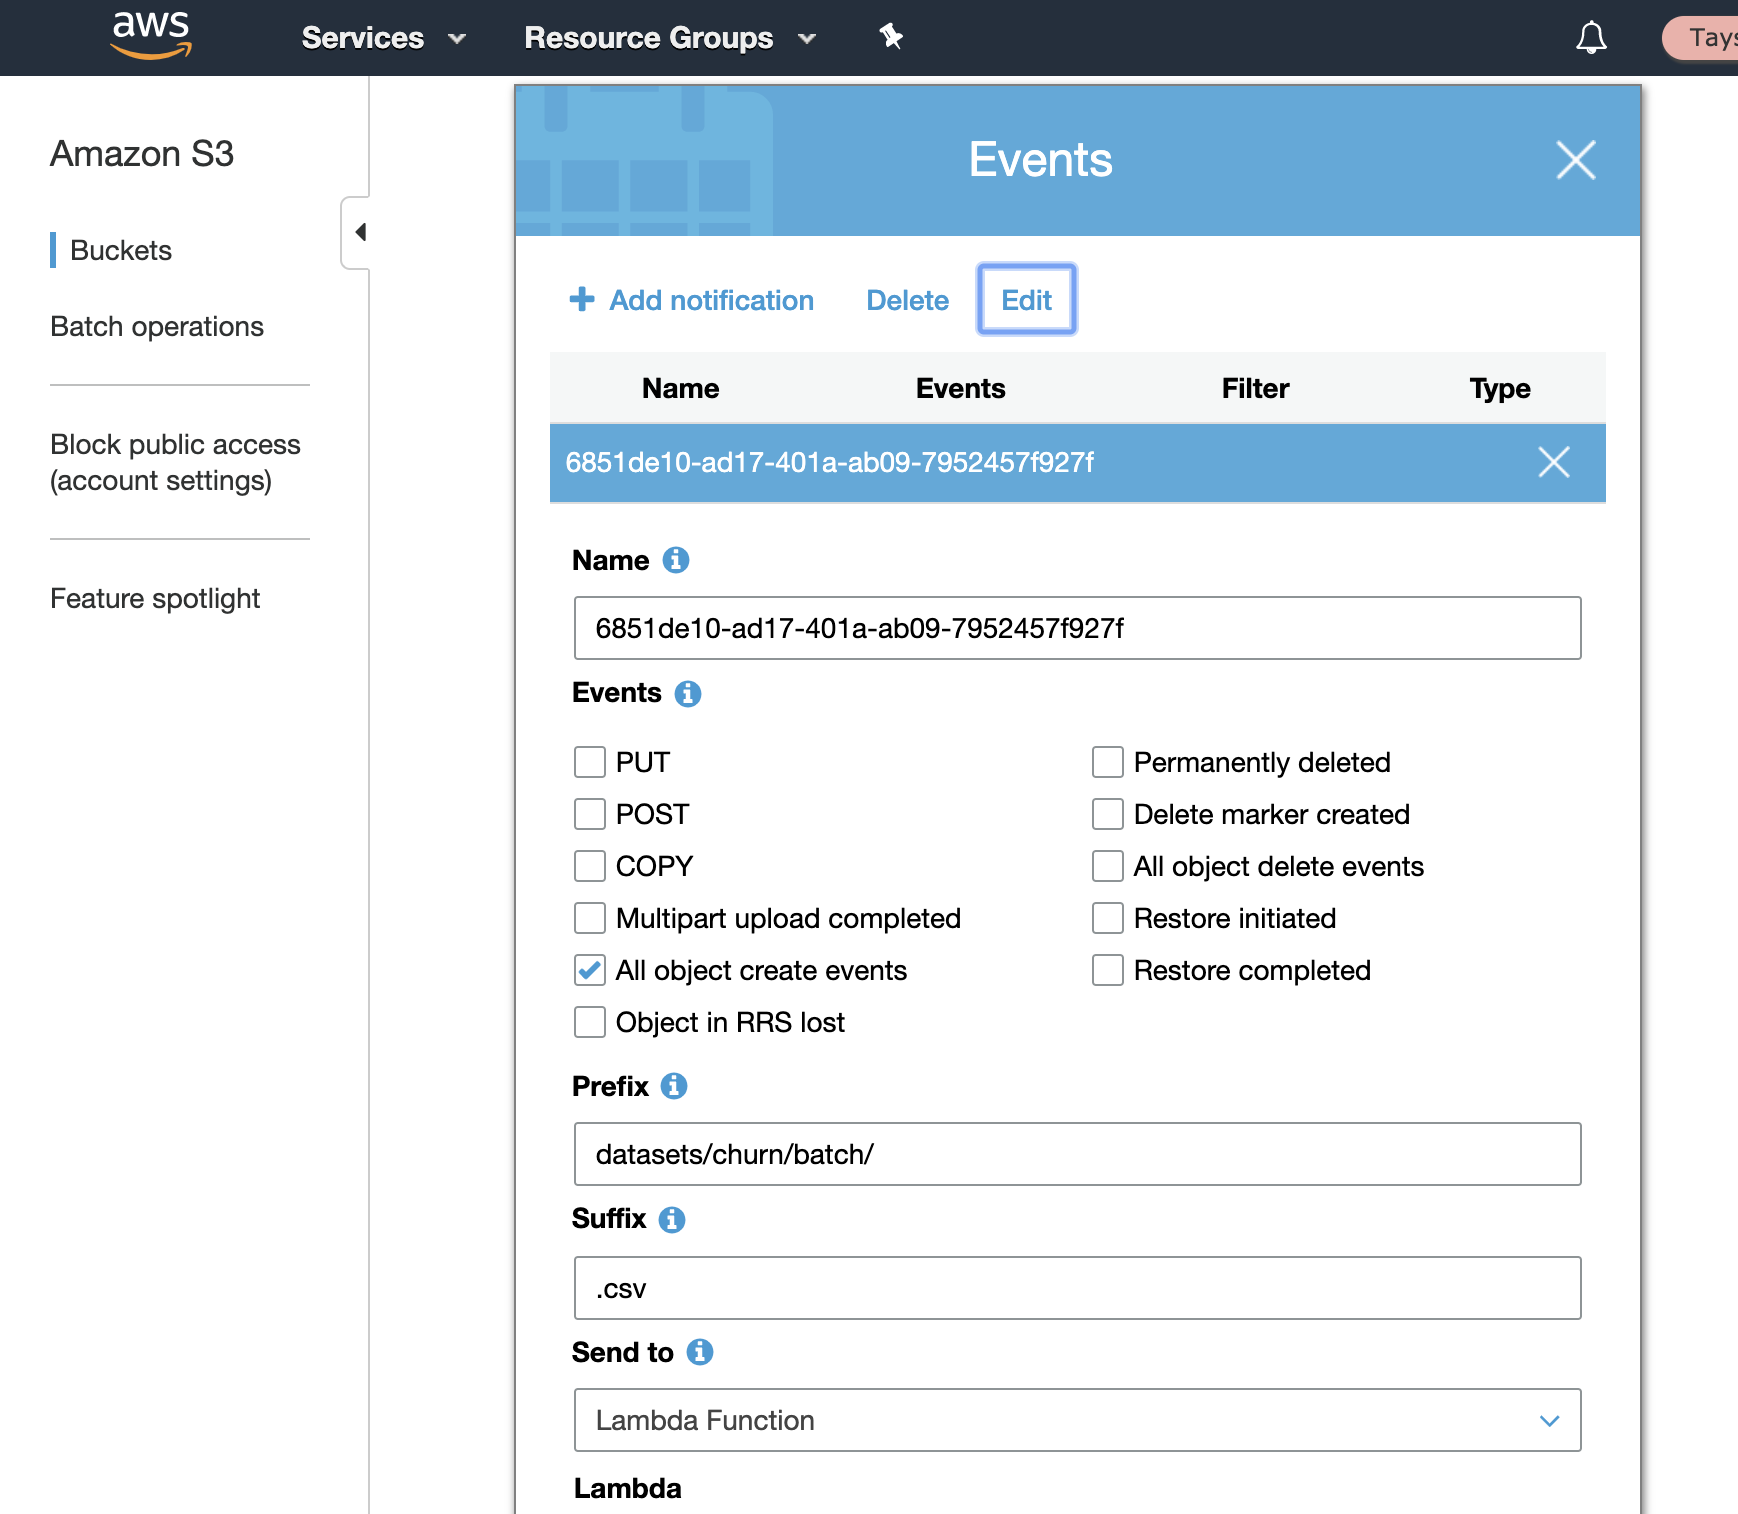
\includegraphics[width=1\linewidth]{S3_bucket_event_2.png}
   \caption{}
   \label{fig:S3_bucket_event_2}
\end{minipage}%
\end{figure}



\subsection{Configure test event}
The event is \textit{dict} type with \textit{JSON} format. The \textbf{test event} is used for debug your Lambda function. See figure \ref{fig:configure_test_event_1}, Select \textbf{Create new test event} and then choose \textbf{Amazon S3 put}.

\begin{figure}[H]
\centering
\begin{minipage}{1\textwidth}
  \centering
  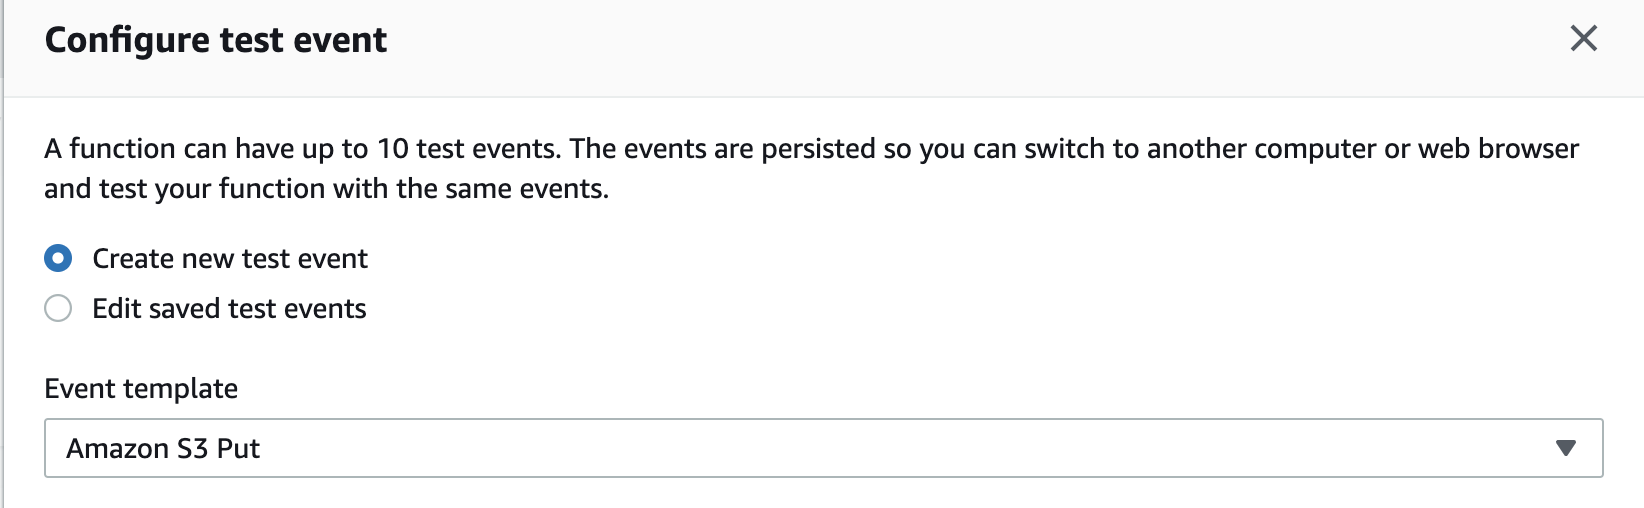
\includegraphics[width=1\linewidth]{configure_test_event_1.png}
   \caption{Add endpoint of model to your Lambda Function}
   \label{fig:configure_test_event_1}
\end{minipage}%
\end{figure}
\noindent
you need to modify \textit{bucket name} and the \textit{key}(the path of your input dataset). For example, the test event used in our case see figure \ref{fig:configure_test_event_2}. 

\begin{figure}[H]
\centering
\begin{minipage}{1\textwidth}
  \centering
  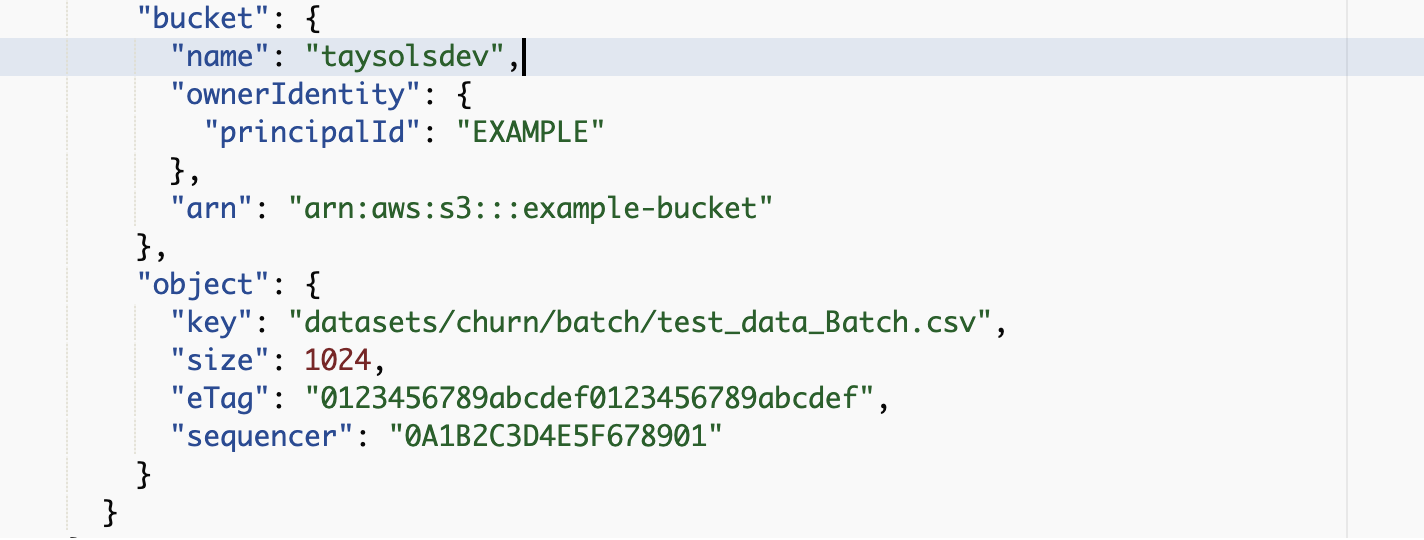
\includegraphics[width=1\linewidth]{configure_test_event_2.png}
   \caption{Modify the content of test event template}
   \label{fig:configure_test_event_2}
\end{minipage}%
\end{figure}


\subsection{Build Lambda Function}

\subsubsection{Lambda Handler with its Help function}

In this example, our main function is \textbf{\textit{lambda\_handler}} within \textbf{\textit{lambda\_function.py}}, see figure \ref{fig:handler_info}
\begin{figure}[H]
\centering
\begin{minipage}{.4\textwidth}
  \centering
  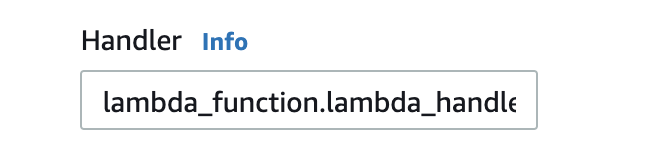
\includegraphics[width=1\linewidth]{handler_info.png}
   \caption{Lambda Handler infomation}
   \label{fig:handler_info}
\end{minipage}%
\end{figure}

To make the main function easy to be understood and modify, I create script \textbf{\textit{help\_function\_lambda.py}} for all necessary help functions used in \textbf{\textit{lambda\_handler}}. These scripts are located in the same folder \textbf{\textit{MyFirstFunction}}\textit{(The name of the lambda function we created)}.


\subsubsection{Lambda Handler Function}
At the time you create a Lambda function, you specify a handler, which is a function in your code, that AWS Lambda can invoke when the service executes your code.I show the example that how to creating a handler function in Python. 
\\
\noindent
In the syntax, note the following:
\begin{enumerate}
\item \textbf{event} – AWS Lambda uses this parameter to pass in event data to the handler. This parameter is usually of the Python \textbf{\textit{dict}} type with \textbf{\textit{JSON}} format. 
\item \textbf{context} – AWS Lambda uses this parameter to provide runtime information to your handler. This parameter is of the \textit{Lambda Context} type.
\item \textbf{runtime.invoke\_endpoint} After you deploy a model into production using Amazon SageMaker hosting services, your client applications use this API to get inferences from the model hosted at the specified endpoint. Parameter \textbf{\textit{EndpointName}}: The name of endpoint of your per-trained model. You can find the endpoint name of your model in Amazon SageMaker interface.
Parameter \textbf{\textit{Body}} (\textit{bytes or seekable file-like object}): Provides input data, Amazon SageMaker passes all of the data in the body to the model. \textit{\textbf{.get()}} returns a \textit{StreamingBody}. This is a series of bytes, not a string, thus we do need \textit{.decode('utf-8')}. \Textbf{Return Type of \textit{invoke\_endpoint}}: See figure \ref{fig:Lambda_function_return_type}\\

\begin{figure}[H]
\centering
\begin{minipage}{1\textwidth}
  \centering
  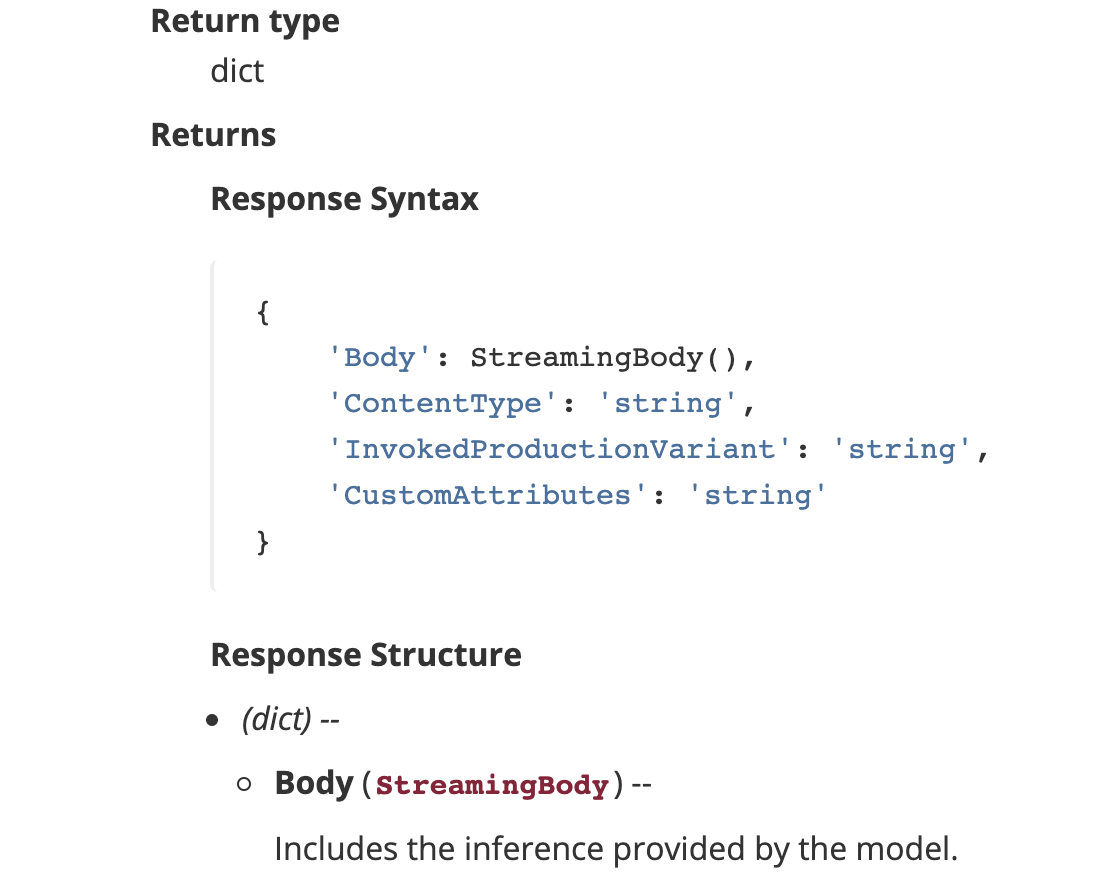
\includegraphics[width=.6\linewidth]{Lambda_function_return_type.png}
   \caption{Invoke Endpoint Return Content}
   \label{fig:Lambda_function_return_type}
\end{minipage}%
\end{figure}
\end{enumerate}

See figure \ref{fig:lambda_handler}

\begin{figure}[H]
\centering
\begin{minipage}{1\textwidth}
  \centering
  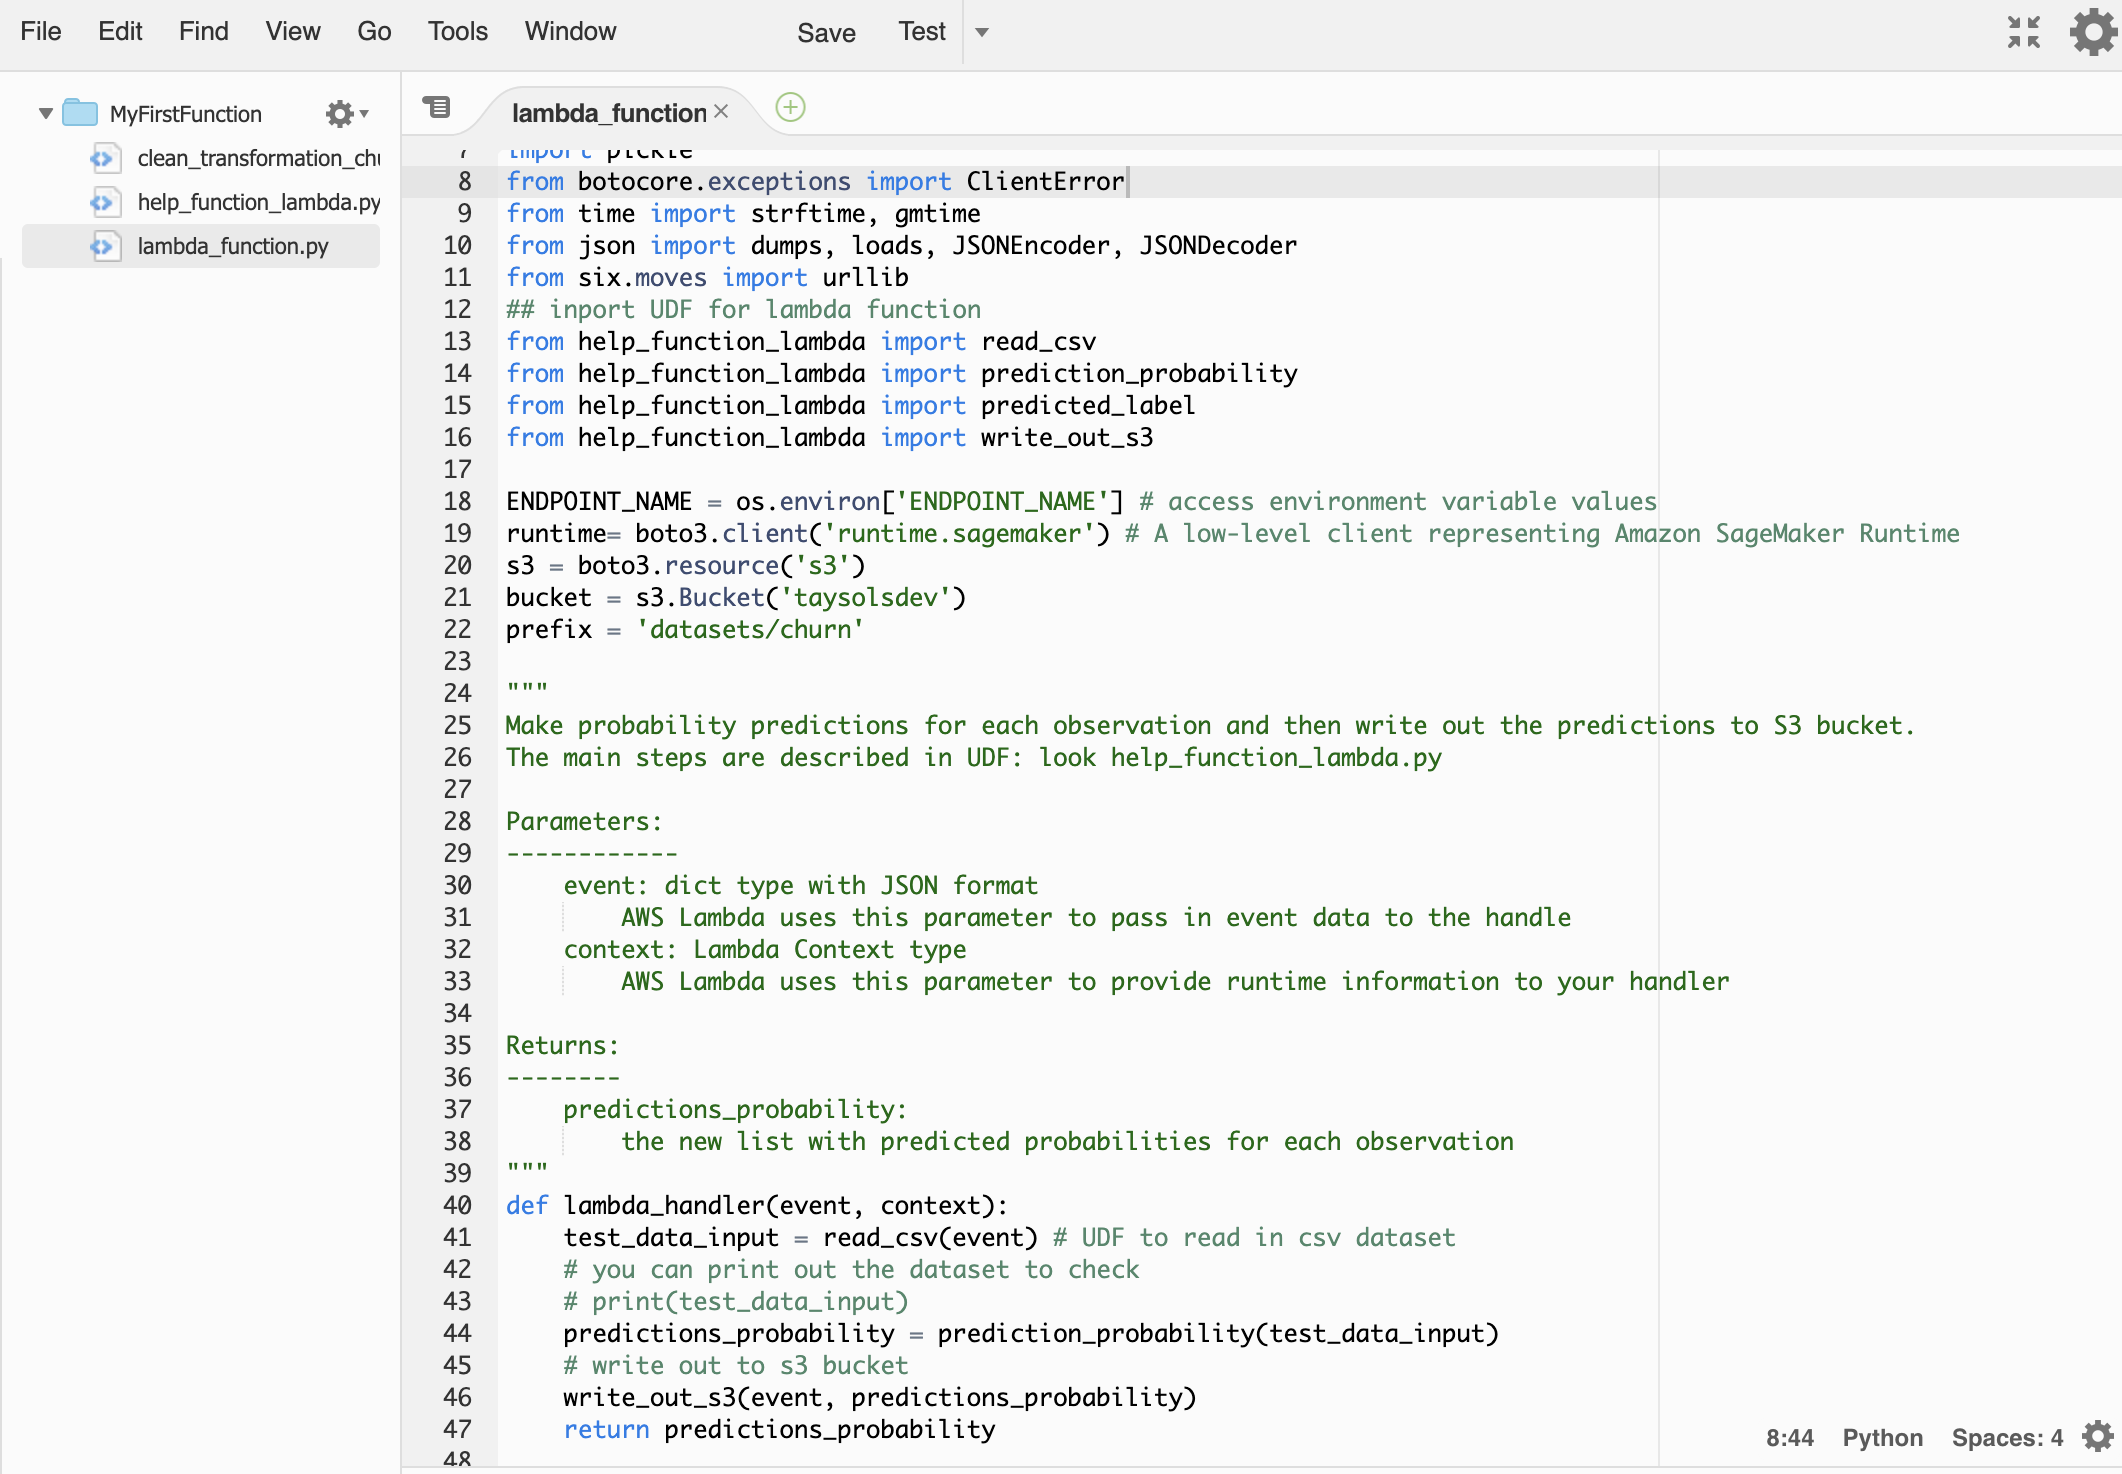
\includegraphics[width=1\linewidth]{lambda_handler.png}
   \caption{Lambda Handler function}
   \label{fig:lambda_handler}
\end{minipage}%
\end{figure}


\subsubsection{Help functions for lambda handler}
To make function easy to be understood and modify, I block functions as followings see figure \ref{fig:help_function_1}, \ref{fig:help_function_2}, \ref{fig:help_function_3}, and \ref{fig:help_function_4}:


\begin{figure}[H]
\centering
\begin{minipage}{1\textwidth}
  \centering
  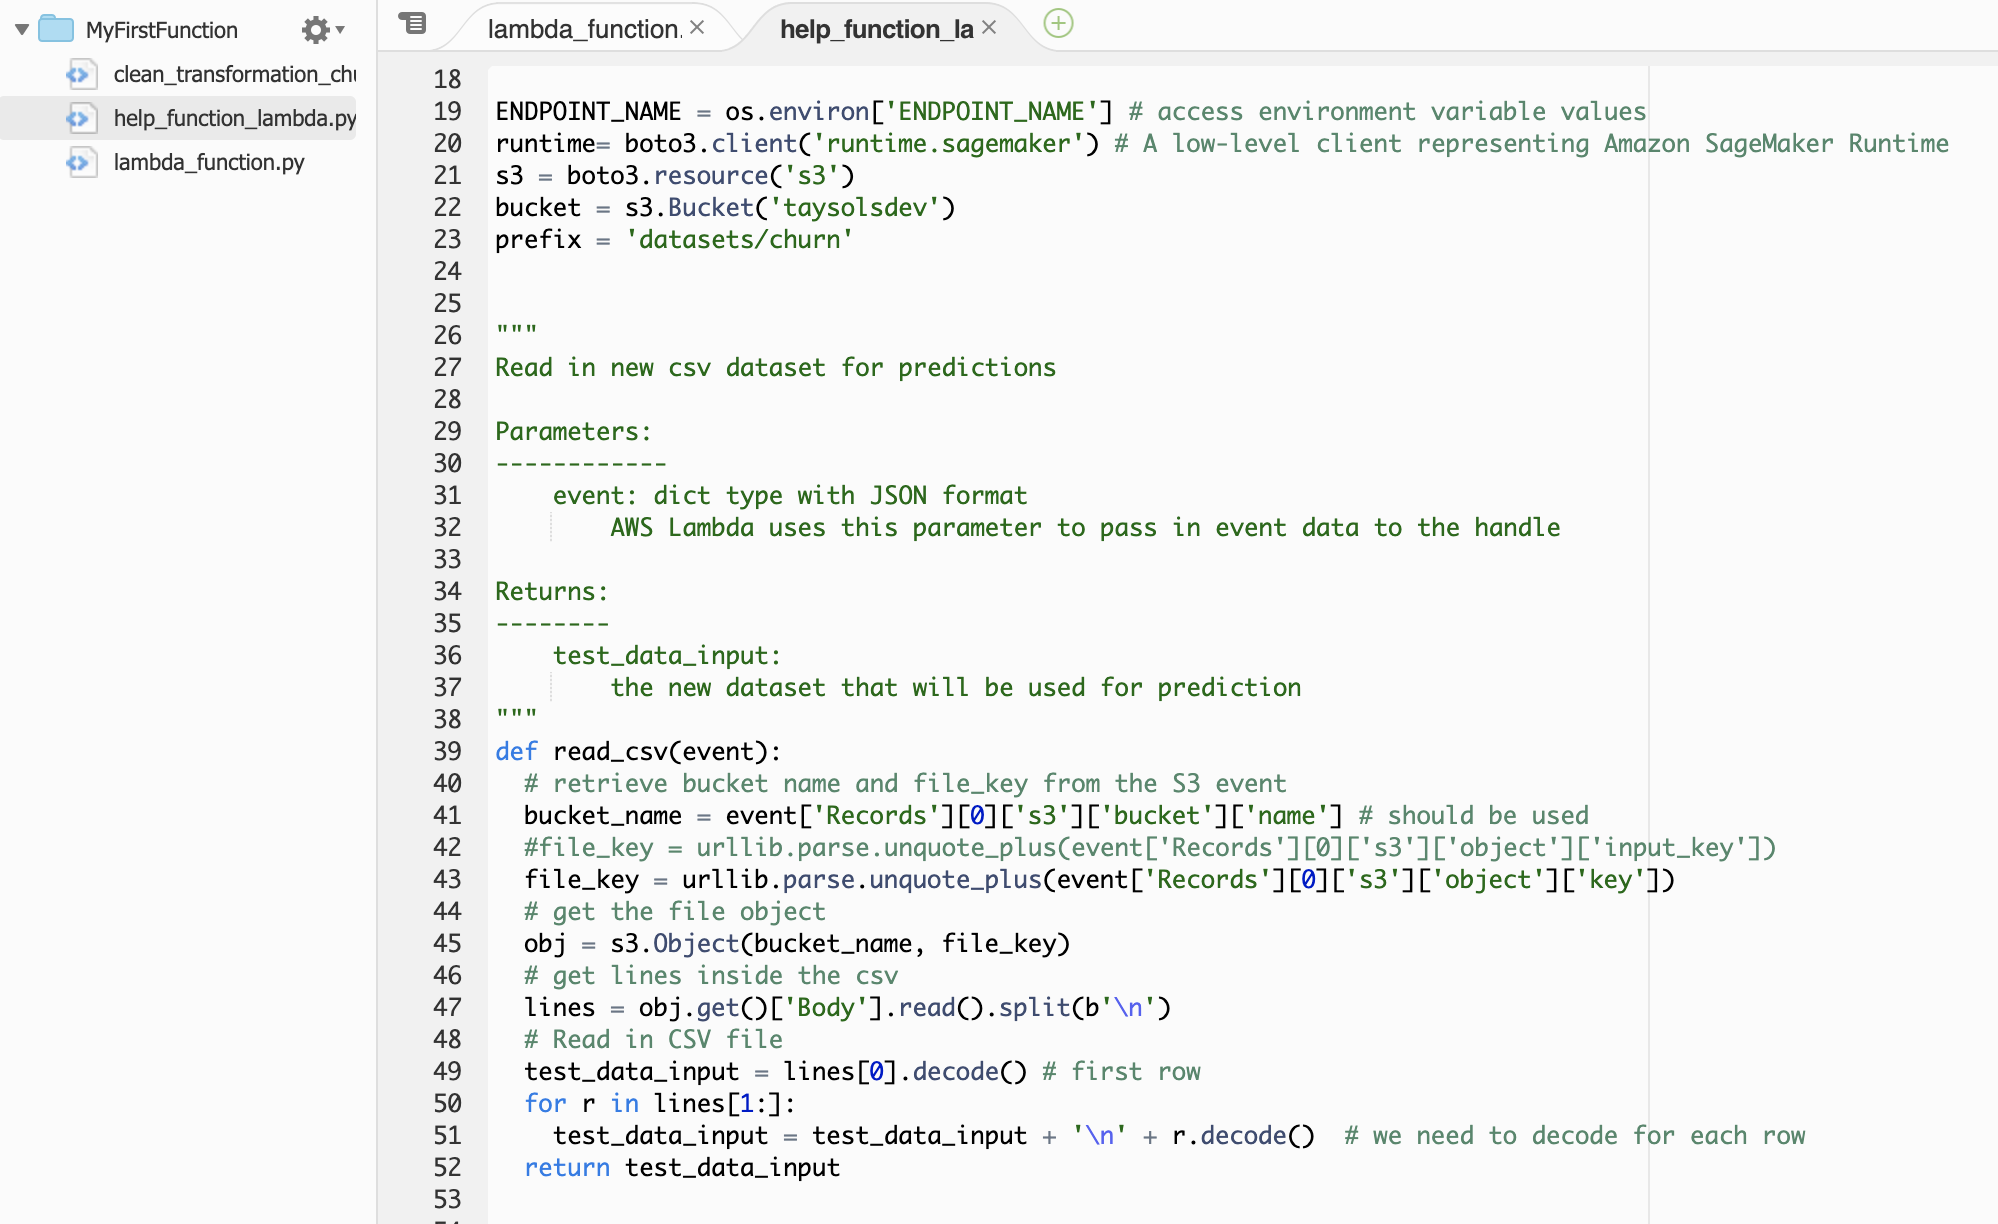
\includegraphics[width=1\linewidth]{help_function_1.png}
   \caption{Read CSV}
   \label{fig:help_function_1}
\end{minipage}%
\end{figure}

\begin{figure}[H]
\centering
\begin{minipage}{1\textwidth}
  \centering
  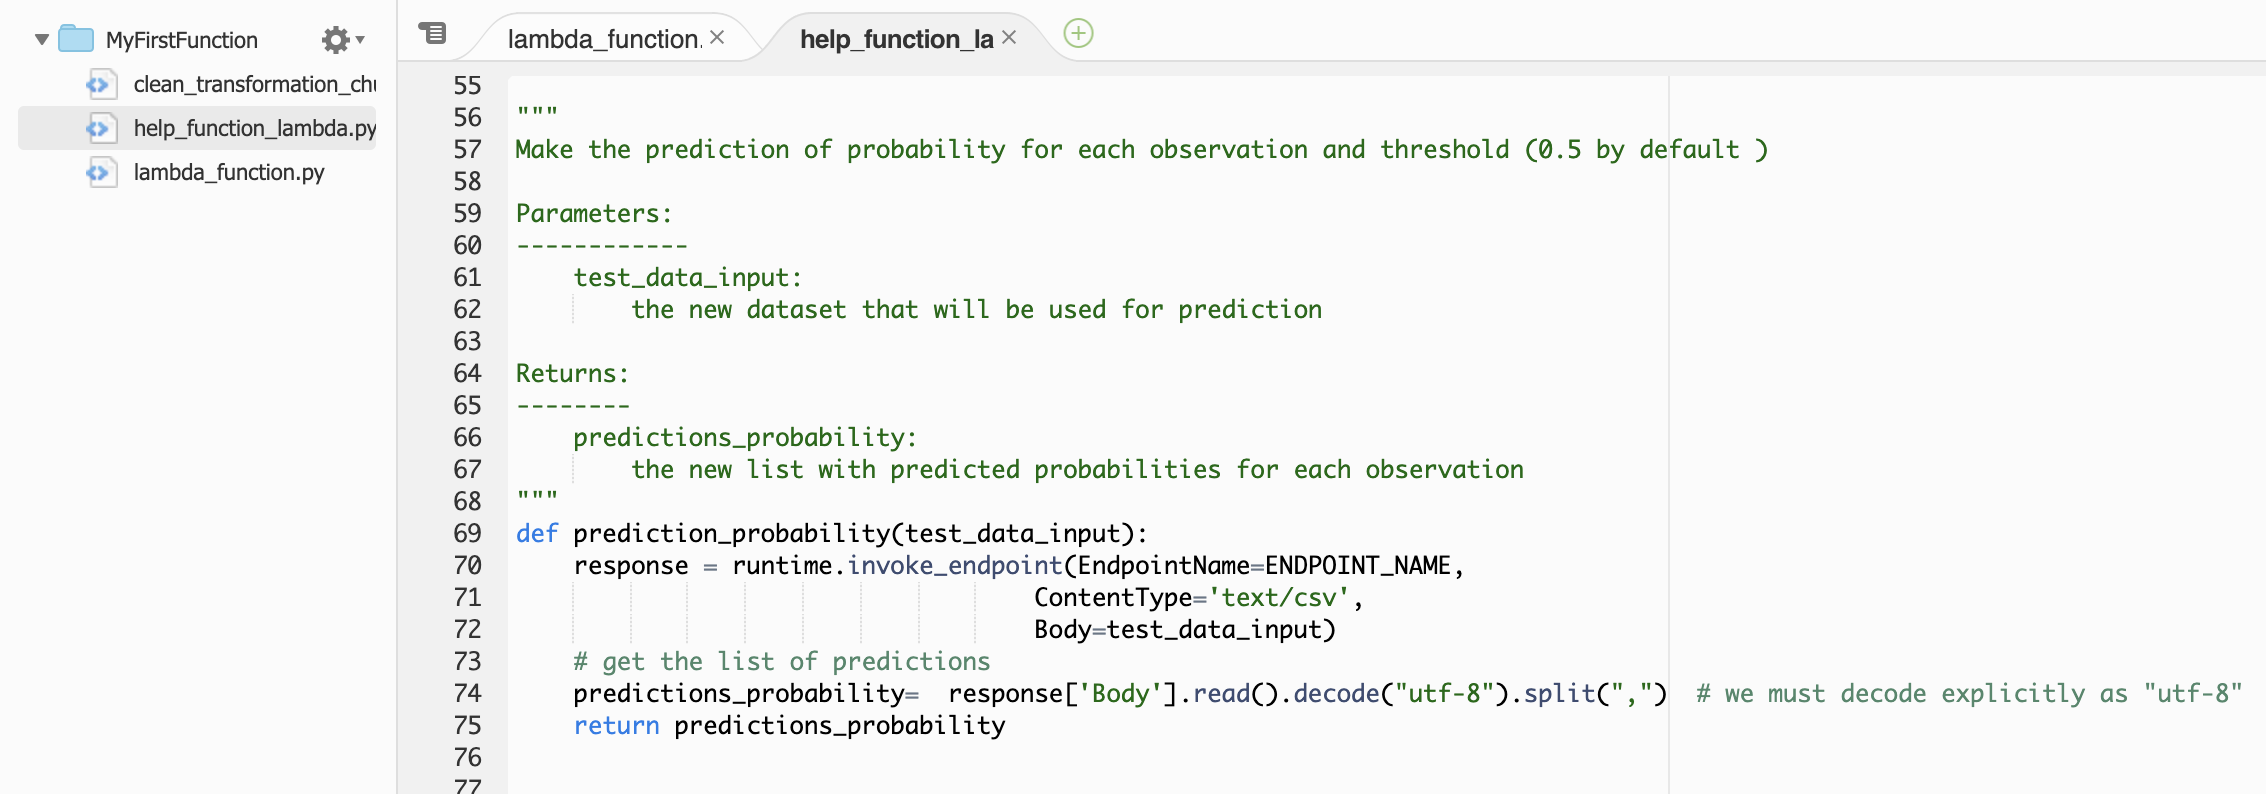
\includegraphics[width=1\linewidth]{help_function_2.png}
   \caption{Probability prediction based on endpoint}
   \label{fig:help_function_2}
\end{minipage}%
\end{figure}

\begin{figure}[H]
\centering
\begin{minipage}{1\textwidth}
  \centering
  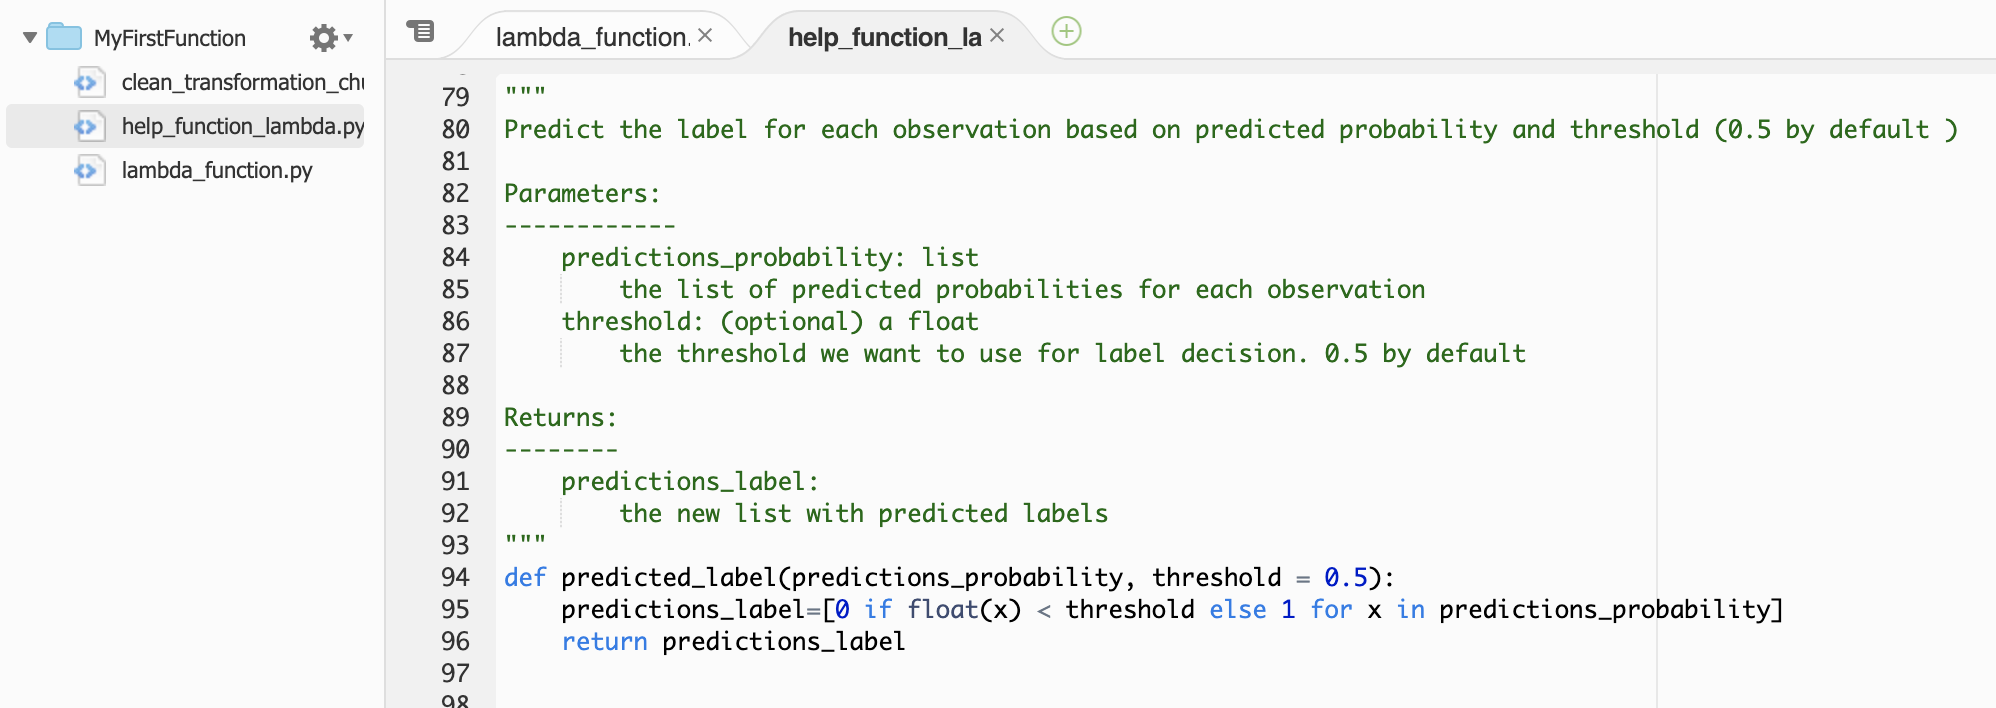
\includegraphics[width=1\linewidth]{help_function_3.png}
   \caption{Label prediction based on threshold}
   \label{fig:help_function_3}
\end{minipage}%
\end{figure}

\begin{figure}[H]
\centering
\begin{minipage}{1\textwidth}
  \centering
  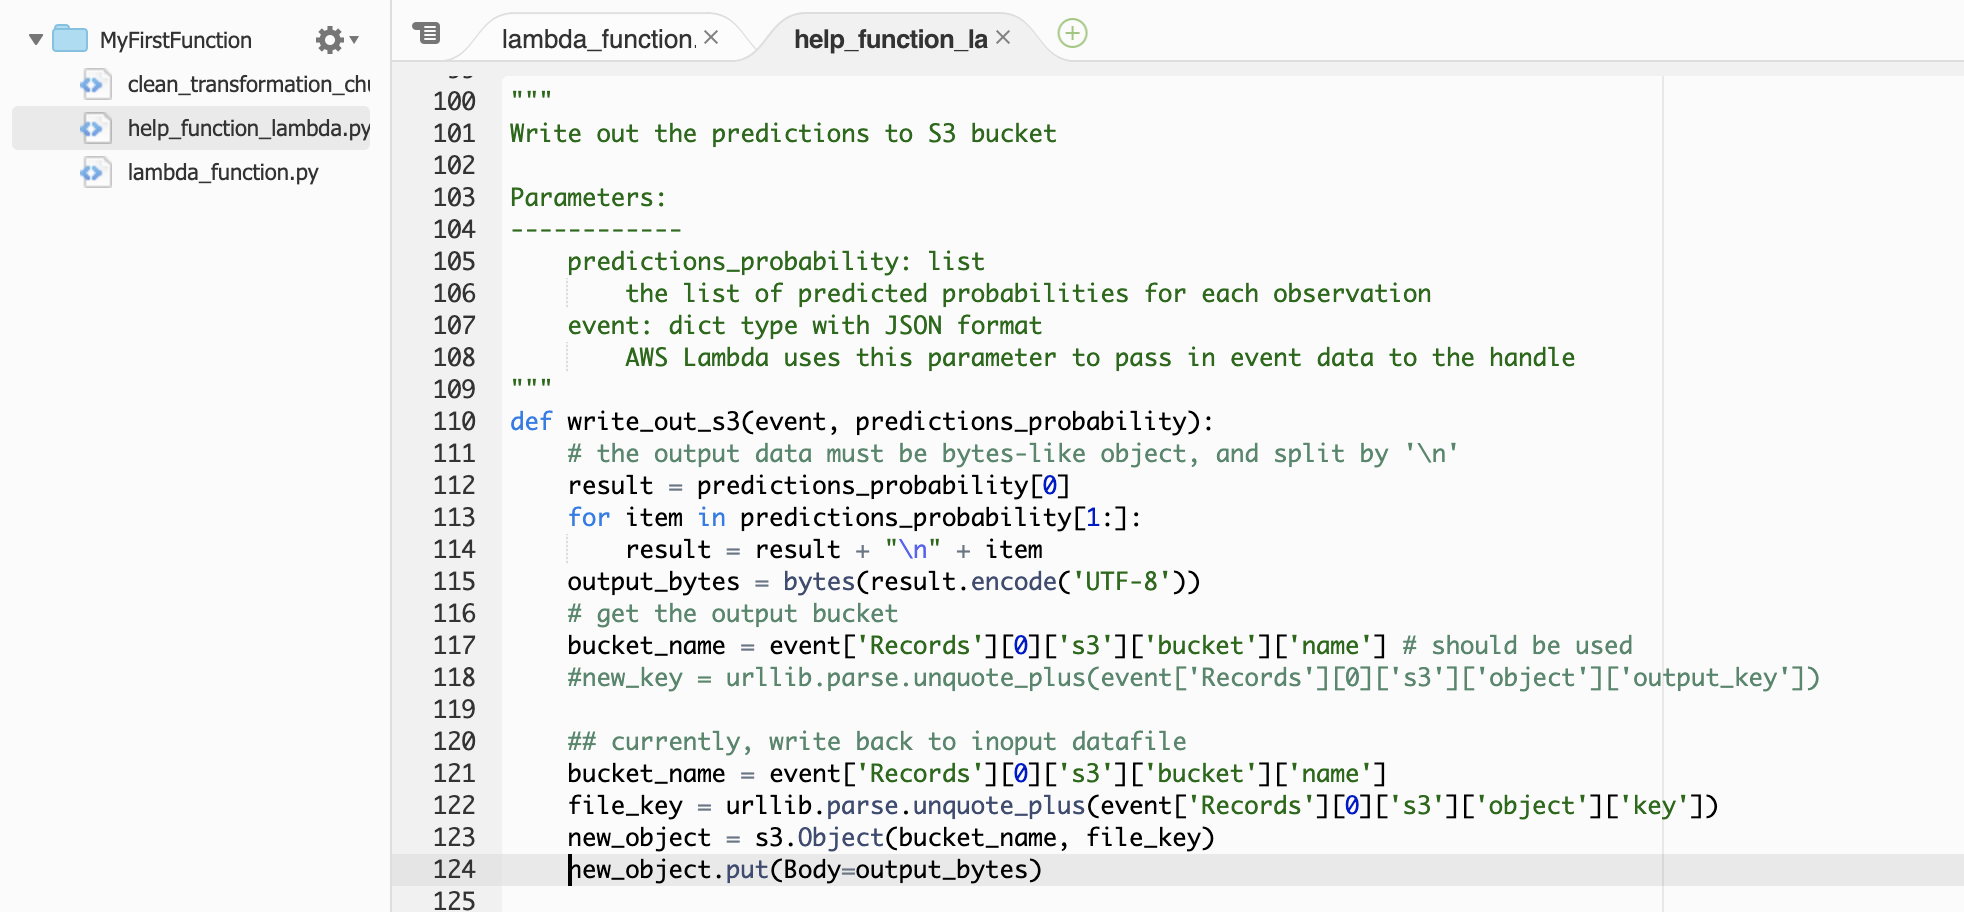
\includegraphics[width=1\linewidth]{help_function_4.png}
   \caption{Write out output to S3 bucket}
   \label{fig:help_function_4}
\end{minipage}%
\end{figure}




\subsection{Common error and the way to fix}
\subsubsection{Configuration is ambiguously defined.}
When you fail to add s3 trigger as \textit{Lambda Error for event source : Configuration is ambiguously defined}, the reason could be that some other lambda function previously using the same trigger was deleted. This does not automatically clear the event notification from the S3 side. You have to \textbf{\textit{navigate to the S3 console and manually delete the stale event notifications}}.
\href{https://forums.aws.amazon.com/thread.jspa?messageID=670712}{\textit{Clink me to read the detail about this error}}


\subsubsection{TypeError: expected string or bytes-like object}
It is the type error you might meet when try to save a Python list to an S3 bucket. In this case, we have to \textbf{convert  list to bytes}. Thus, we need \textit{bytes(json.dumps(predictions_probability, indent=2).encode('UTF-8')))}




\newpage
\section{Test data: Check CloudWatch}

By default, Lambda will write function activity to CloudWatch. This is why the role that was created earlier had to get access to CloudWatch. When a new file is uploaded to the S3 bucket that has the subscribed event, this should automatically kick off the Lambda function. To confirm this, head over to CloudWatch or click on the Monitoring tab inside of the function itself. 

\\
\noindent
It is important to know how to look \textbf{CloudWatch Logs Insights} to check if the event (for example, inpout data to S3 in our case) trigger the Lambda function successfully, and if fail, you can read the error information here to debug.











\newpage
\section{Reference}

\begin{enumerate}
\item \url{https://aws.amazon.com/cn/blogs/machine-learning/call-an-amazon-sagemaker-model-endpoint-using-amazon-api-gateway-and-aws-lambda/}

\item \url{https://n2ws.com/blog/aws-automation/lambda-function-s3-event-triggers}


\end{enumerate}






\setlength{\parskip}{1em}
\end{document}

